\documentclass[a4paper]{book}
\usepackage{makeidx}
\usepackage{graphicx}
\usepackage{multicol}
\usepackage{float}
\usepackage{listings}
\usepackage{color}
\usepackage{textcomp}
\usepackage{alltt}
\usepackage{times}
\usepackage{ifpdf}
\ifpdf
\usepackage[pdftex,
            pagebackref=true,
            colorlinks=true,
            linkcolor=blue,
            unicode
           ]{hyperref}
\else
\usepackage[ps2pdf,
            pagebackref=true,
            colorlinks=true,
            linkcolor=blue,
            unicode
           ]{hyperref}
\usepackage{pspicture}
\fi
\usepackage[utf8]{inputenc}
\usepackage{doxygen}
\lstset{language=C++,inputencoding=utf8,basicstyle=\footnotesize,breaklines=true,breakatwhitespace=true,tabsize=4,numbers=left }
\makeindex
\setcounter{tocdepth}{3}
\renewcommand{\footrulewidth}{0.4pt}
\begin{document}
\hypersetup{pageanchor=false}
\begin{titlepage}
\vspace*{7cm}
\begin{center}
{\Large Ball Game }\\
\vspace*{1cm}
{\large Generated by Doxygen 1.6.1}\\
\vspace*{0.5cm}
{\small Mon May 4 23:02:03 2015}\\
\end{center}
\end{titlepage}
\clearemptydoublepage
\pagenumbering{roman}
\tableofcontents
\clearemptydoublepage
\pagenumbering{arabic}
\hypersetup{pageanchor=true}
\chapter{Class Index}
\section{Class Hierarchy}
This inheritance list is sorted roughly, but not completely, alphabetically:\begin{DoxyCompactList}
\item \contentsline{section}{Ball}{\pageref{structBall}}{}
\item \contentsline{section}{BallControl}{\pageref{classBallControl}}{}
\begin{DoxyCompactList}
\item \contentsline{section}{ColorTransferControl}{\pageref{classColorTransferControl}}{}
\end{DoxyCompactList}
\item \contentsline{section}{BallGrid}{\pageref{classBallGrid}}{}
\item \contentsline{section}{BallRenderer}{\pageref{classBallRenderer}}{}
\begin{DoxyCompactList}
\item \contentsline{section}{PropulsionBallRenderer}{\pageref{classPropulsionBallRenderer}}{}
\item \contentsline{section}{VelocityBallRendererX}{\pageref{classVelocityBallRendererX}}{}
\item \contentsline{section}{VelocityBallRendererY}{\pageref{classVelocityBallRendererY}}{}
\end{DoxyCompactList}
\item \contentsline{section}{BallSpawnSystem}{\pageref{structBallSpawnSystem}}{}
\item \contentsline{section}{Randini::Camera2D}{\pageref{classRandini_1_1Camera2D}}{}
\item \contentsline{section}{Cell}{\pageref{structCell}}{}
\item \contentsline{section}{Randini::ColorRGBA8}{\pageref{structRandini_1_1ColorRGBA8}}{}
\item \contentsline{section}{Randini::FPSLimiter}{\pageref{classRandini_1_1FPSLimiter}}{}
\item \contentsline{section}{Randini::GLSLProgram}{\pageref{classRandini_1_1GLSLProgram}}{}
\item \contentsline{section}{Randini::GLTexture}{\pageref{structRandini_1_1GLTexture}}{}
\item \contentsline{section}{Randini::Glyph}{\pageref{classRandini_1_1Glyph}}{}
\item \contentsline{section}{Randini::ImageLoader}{\pageref{classRandini_1_1ImageLoader}}{}
\item \contentsline{section}{Randini::InputControl}{\pageref{classRandini_1_1InputControl}}{}
\item \contentsline{section}{Randini::IOManager}{\pageref{classRandini_1_1IOManager}}{}
\item \contentsline{section}{MainGame}{\pageref{classMainGame}}{}
\item \contentsline{section}{Randini::Position}{\pageref{structRandini_1_1Position}}{}
\item \contentsline{section}{Randini::RenderLoader}{\pageref{classRandini_1_1RenderLoader}}{}
\item \contentsline{section}{Randini::ResourceManager}{\pageref{classRandini_1_1ResourceManager}}{}
\item \contentsline{section}{Randini::SpriteLoader}{\pageref{classRandini_1_1SpriteLoader}}{}
\item \contentsline{section}{Randini::TextureCache}{\pageref{classRandini_1_1TextureCache}}{}
\item \contentsline{section}{Randini::UV}{\pageref{structRandini_1_1UV}}{}
\item \contentsline{section}{Randini::Vertex}{\pageref{structRandini_1_1Vertex}}{}
\item \contentsline{section}{Randini::Window}{\pageref{classRandini_1_1Window}}{}
\end{DoxyCompactList}

\chapter{Class Index}
\section{Class List}
Here are the classes, structs, unions and interfaces with brief descriptions:\begin{DoxyCompactList}
\item\contentsline{section}{\hyperlink{structBall}{Ball} }{\pageref{structBall}}{}
\item\contentsline{section}{\hyperlink{classBallControl}{BallControl} }{\pageref{classBallControl}}{}
\item\contentsline{section}{\hyperlink{classBallGrid}{BallGrid} }{\pageref{classBallGrid}}{}
\item\contentsline{section}{\hyperlink{classBallRenderer}{BallRenderer} }{\pageref{classBallRenderer}}{}
\item\contentsline{section}{\hyperlink{structBallSpawnSystem}{BallSpawnSystem} }{\pageref{structBallSpawnSystem}}{}
\item\contentsline{section}{\hyperlink{classRandini_1_1Camera2D}{Randini::Camera2D} }{\pageref{classRandini_1_1Camera2D}}{}
\item\contentsline{section}{\hyperlink{structCell}{Cell} (Inlcude vector as using vector for the list )}{\pageref{structCell}}{}
\item\contentsline{section}{\hyperlink{structRandini_1_1ColorRGBA8}{Randini::ColorRGBA8} }{\pageref{structRandini_1_1ColorRGBA8}}{}
\item\contentsline{section}{\hyperlink{classColorTransferControl}{ColorTransferControl} }{\pageref{classColorTransferControl}}{}
\item\contentsline{section}{\hyperlink{classRandini_1_1FPSLimiter}{Randini::FPSLimiter} }{\pageref{classRandini_1_1FPSLimiter}}{}
\item\contentsline{section}{\hyperlink{classRandini_1_1GLSLProgram}{Randini::GLSLProgram} }{\pageref{classRandini_1_1GLSLProgram}}{}
\item\contentsline{section}{\hyperlink{structRandini_1_1GLTexture}{Randini::GLTexture} (The \hyperlink{structRandini_1_1GLTexture}{GLTexture} struct make is for the id of the texture as well as width and height to know the properties of the texture )}{\pageref{structRandini_1_1GLTexture}}{}
\item\contentsline{section}{\hyperlink{classRandini_1_1Glyph}{Randini::Glyph} }{\pageref{classRandini_1_1Glyph}}{}
\item\contentsline{section}{\hyperlink{classRandini_1_1ImageLoader}{Randini::ImageLoader} }{\pageref{classRandini_1_1ImageLoader}}{}
\item\contentsline{section}{\hyperlink{classRandini_1_1InputControl}{Randini::InputControl} (The \hyperlink{classRandini_1_1InputControl}{InputControl} class Overall stores a key map which maps SDL\_\-Keys to bools If the value is true this means the key has been pressed Anything else means the key has been released )}{\pageref{classRandini_1_1InputControl}}{}
\item\contentsline{section}{\hyperlink{classRandini_1_1IOManager}{Randini::IOManager} }{\pageref{classRandini_1_1IOManager}}{}
\item\contentsline{section}{\hyperlink{classMainGame}{MainGame} }{\pageref{classMainGame}}{}
\item\contentsline{section}{\hyperlink{structRandini_1_1Position}{Randini::Position} }{\pageref{structRandini_1_1Position}}{}
\item\contentsline{section}{\hyperlink{classPropulsionBallRenderer}{PropulsionBallRenderer} (\hyperlink{classPropulsionBallRenderer}{PropulsionBallRenderer} The \hyperlink{classPropulsionBallRenderer}{PropulsionBallRenderer} class When balls increase in velocity they become brighter Set new renderer using same elements from renderBalls but altered inherits the virtual function )}{\pageref{classPropulsionBallRenderer}}{}
\item\contentsline{section}{\hyperlink{classRandini_1_1RenderLoader}{Randini::RenderLoader} }{\pageref{classRandini_1_1RenderLoader}}{}
\item\contentsline{section}{\hyperlink{classRandini_1_1ResourceManager}{Randini::ResourceManager} }{\pageref{classRandini_1_1ResourceManager}}{}
\item\contentsline{section}{\hyperlink{classRandini_1_1SpriteLoader}{Randini::SpriteLoader} }{\pageref{classRandini_1_1SpriteLoader}}{}
\item\contentsline{section}{\hyperlink{classRandini_1_1TextureCache}{Randini::TextureCache} }{\pageref{classRandini_1_1TextureCache}}{}
\item\contentsline{section}{\hyperlink{structRandini_1_1UV}{Randini::UV} }{\pageref{structRandini_1_1UV}}{}
\item\contentsline{section}{\hyperlink{classVelocityBallRendererX}{VelocityBallRendererX} (The \hyperlink{classVelocityBallRendererX}{VelocityBallRendererX} class Visualise the velocity of ball renderers when moving in the x direction as well as visualise the position with different colours )}{\pageref{classVelocityBallRendererX}}{}
\item\contentsline{section}{\hyperlink{classVelocityBallRendererY}{VelocityBallRendererY} (The \hyperlink{classVelocityBallRendererY}{VelocityBallRendererY} class Visualise the velocity of ball renderers when moving in the y direction as well as visualise the position with different colours )}{\pageref{classVelocityBallRendererY}}{}
\item\contentsline{section}{\hyperlink{structRandini_1_1Vertex}{Randini::Vertex} }{\pageref{structRandini_1_1Vertex}}{}
\item\contentsline{section}{\hyperlink{classRandini_1_1Window}{Randini::Window} }{\pageref{classRandini_1_1Window}}{}
\end{DoxyCompactList}

\chapter{File Index}
\section{File List}
Here is a list of all documented files with brief descriptions:\begin{DoxyCompactList}
\item\contentsline{section}{Include/BallGame/\hyperlink{Ball_8h}{Ball.h} (Handle the data for the ball )}{\pageref{Ball_8h}}{}
\item\contentsline{section}{Include/BallGame/\hyperlink{BallControl_8h}{BallControl.h} (Handle different ball controls and tracks mouse for grabbing )}{\pageref{BallControl_8h}}{}
\item\contentsline{section}{Include/BallGame/\hyperlink{BallGrid_8h}{BallGrid.h} (Imports the grid/cells to store balls in for spatial partioning )}{\pageref{BallGrid_8h}}{}
\item\contentsline{section}{Include/BallGame/\hyperlink{BallRenderer_8h}{BallRenderer.h} (Contolrs different renders and inits the shaders and textures )}{\pageref{BallRenderer_8h}}{}
\item\contentsline{section}{Include/BallGame/\hyperlink{MainGame_8h}{MainGame.h} (Calls functions from Randini Engine \& deals with key input, drawing, deltatime )}{\pageref{MainGame_8h}}{}
\item\contentsline{section}{Include/Randini/\hyperlink{Camera2D_8h}{Camera2D.h} (Creates the camera gains screen coordinates and returns the camera position )}{\pageref{Camera2D_8h}}{}
\item\contentsline{section}{Include/Randini/{\bfseries Errors.h} }{\pageref{Errors_8h}}{}
\item\contentsline{section}{Include/Randini/\hyperlink{GLSLProgram_8h}{GLSLProgram.h} (Compiles, Links, Enables, \& Disables frag and vert shaders and returns the location of the uniform )}{\pageref{GLSLProgram_8h}}{}
\item\contentsline{section}{Include/Randini/\hyperlink{GLTexture_8h}{GLTexture.h} (Creats a struct to handle data id of textures )}{\pageref{GLTexture_8h}}{}
\item\contentsline{section}{Include/Randini/\hyperlink{ImageLoader_8h}{ImageLoader.h} (Reads a texture file and returns a GLTexture )}{\pageref{ImageLoader_8h}}{}
\item\contentsline{section}{Include/Randini/{\bfseries InputControl.h} }{\pageref{InputControl_8h}}{}
\item\contentsline{section}{Include/Randini/\hyperlink{IOManager_8h}{IOManager.h} (Seeks the size of the buffer and reads the file to it returns open file )}{\pageref{IOManager_8h}}{}
\item\contentsline{section}{Include/Randini/{\bfseries picoPNG.h} }{\pageref{picoPNG_8h}}{}
\item\contentsline{section}{Include/Randini/\hyperlink{Randini_8h}{Randini.h} (Encapsulates all data in namespace, inits everything and sets double buffer )}{\pageref{Randini_8h}}{}
\item\contentsline{section}{Include/Randini/\hyperlink{ResourceManager_8h}{ResourceManager.h} (Calls texturecache to retrieve texture path )}{\pageref{ResourceManager_8h}}{}
\item\contentsline{section}{Include/Randini/\hyperlink{SpriteLoader_8h}{SpriteLoader.h} (Allows for multiple sprites to be drawn \& rendered. Sets vertices for glyphs )}{\pageref{SpriteLoader_8h}}{}
\item\contentsline{section}{Include/Randini/\hyperlink{TextureCache_8h}{TextureCache.h} (Checks if texture is in texture map, loads new textures and creates new path. Returns new texture )}{\pageref{TextureCache_8h}}{}
\item\contentsline{section}{Include/Randini/\hyperlink{Timer_8h}{Timer.h} (Calculates, monitors, and caps the FPS this allows for setting deltaTime later )}{\pageref{Timer_8h}}{}
\item\contentsline{section}{Include/Randini/\hyperlink{Vertex_8h}{Vertex.h} (Handle the data for the ball )}{\pageref{Vertex_8h}}{}
\item\contentsline{section}{Include/Randini/\hyperlink{Window_8h}{Window.h} (Creates the genral SDL handles for settign a window, Swaps buffers and assigns window flags )}{\pageref{Window_8h}}{}
\item\contentsline{section}{src/Randini/\hyperlink{Camera2D_8cpp}{Camera2D.cpp} (Implements the camera and retrives the screen coordinates )}{\pageref{Camera2D_8cpp}}{}
\item\contentsline{section}{src/Randini/\hyperlink{Errors_8cpp}{Errors.cpp} (Implements error checking for all classes )}{\pageref{Errors_8cpp}}{}
\item\contentsline{section}{src/Randini/\hyperlink{GLSLProgram_8cpp}{GLSLProgram.cpp} (Compiles, Links and implements shader information and retives uniform location )}{\pageref{GLSLProgram_8cpp}}{}
\item\contentsline{section}{src/Randini/\hyperlink{ImageLoader_8cpp}{ImageLoader.cpp} (Reads/Loads PNG file to output data needed for textures )}{\pageref{ImageLoader_8cpp}}{}
\item\contentsline{section}{src/Randini/\hyperlink{InputControl_8cpp}{InputControl.cpp} (Stores SDL\_\-keys in keymap creating smoother controls )}{\pageref{InputControl_8cpp}}{}
\item\contentsline{section}{src/Randini/\hyperlink{IOManager_8cpp}{IOManager.cpp} (Searches for the size of the buffer and returns erro if it fails )}{\pageref{IOManager_8cpp}}{}
\item\contentsline{section}{src/Randini/\hyperlink{Randini_8cpp}{Randini.cpp} (Encapsulates program in namespace and inits everything )}{\pageref{Randini_8cpp}}{}
\item\contentsline{section}{src/Randini/\hyperlink{ResourceManager_8cpp}{ResourceManager.cpp} (Calls texture chache in order to retrive texture path )}{\pageref{ResourceManager_8cpp}}{}
\item\contentsline{section}{src/Randini/\hyperlink{TextureCache_8cpp}{TextureCache.cpp} (Check if texture is in texture path and creates if there isnt )}{\pageref{TextureCache_8cpp}}{}
\item\contentsline{section}{src/Randini/\hyperlink{Timer_8cpp}{Timer.cpp} (Calculates FPS and ticks then procceeds to cap it at 60 )}{\pageref{Timer_8cpp}}{}
\item\contentsline{section}{src/Randini/\hyperlink{Window_8cpp}{Window.cpp} (Creates the window and allows handles to be manipulated )}{\pageref{Window_8cpp}}{}
\item\contentsline{section}{src/Uni/\hyperlink{Ball_8cpp}{Ball.cpp} (Stores the data for the balls )}{\pageref{Ball_8cpp}}{}
\item\contentsline{section}{src/Uni/\hyperlink{BallControl_8cpp}{BallControl.cpp} (Sets up multiple controls for the ball and deals with wall collision )}{\pageref{BallControl_8cpp}}{}
\item\contentsline{section}{src/Uni/\hyperlink{BallGrid_8cpp}{BallGrid.cpp} (Implements 2D grid and stores balls in cells to allow spatial partioning )}{\pageref{BallGrid_8cpp}}{}
\item\contentsline{section}{src/Uni/\hyperlink{BallRenderer_8cpp}{BallRenderer.cpp} (Outputs different rederers, applys shaders to the balls and renders all the balls )}{\pageref{BallRenderer_8cpp}}{}
\item\contentsline{section}{src/Uni/\hyperlink{MainGame_8cpp}{MainGame.cpp} (Calls certain files from game engine. Deals with user input and spawsn the balls )}{\pageref{MainGame_8cpp}}{}
\end{DoxyCompactList}

\chapter{Class Documentation}
\hypertarget{structBall}{
\section{Ball Struct Reference}
\label{structBall}\index{Ball@{Ball}}
}
\subsection*{Public Member Functions}
\begin{DoxyCompactItemize}
\item 
\hyperlink{structBall_a39a1cb33a6f2e3a4c692144967c3f4ef}{Ball} (float \_\-radius, float \_\-mass, const glm::vec2 \&c\_\-position, const glm::vec2 \&c\_\-velocity, unsigned int \_\-textureId, const \hyperlink{structRandini_1_1ColorRGBA8}{Randini::ColorRGBA8} \&c\_\-color)
\begin{DoxyCompactList}\small\item\em \hyperlink{structBall}{Ball} This struct simply contains all the data for the ball. \item\end{DoxyCompactList}\end{DoxyCompactItemize}
\subsection*{Public Attributes}
\begin{DoxyCompactItemize}
\item 
\hypertarget{structBall_a3bc6acf9f3013d514e9a74c06a81f0cc}{
float {\bfseries m\_\-radius}}
\label{structBall_a3bc6acf9f3013d514e9a74c06a81f0cc}

\item 
\hypertarget{structBall_a22c5fc77318cc724a5e7aad38df1ce85}{
float {\bfseries m\_\-mass}}
\label{structBall_a22c5fc77318cc724a5e7aad38df1ce85}

\item 
\hypertarget{structBall_a5daf4402dc74b3da7806549c120344bd}{
glm::vec2 {\bfseries m\_\-position}}
\label{structBall_a5daf4402dc74b3da7806549c120344bd}

\item 
\hypertarget{structBall_a9537fb69d4b0e4370e3aba2f6b894579}{
glm::vec2 {\bfseries m\_\-velocity}}
\label{structBall_a9537fb69d4b0e4370e3aba2f6b894579}

\item 
\hypertarget{structBall_a9abd8e7caf65e1e6b96cbc101eb95ac5}{
unsigned int {\bfseries m\_\-textureId}}
\label{structBall_a9abd8e7caf65e1e6b96cbc101eb95ac5}

\item 
\hypertarget{structBall_aa8b1fa3be1200bb682524c230e424542}{
\hyperlink{structRandini_1_1ColorRGBA8}{Randini::ColorRGBA8} {\bfseries m\_\-color}}
\label{structBall_aa8b1fa3be1200bb682524c230e424542}

\item 
\hypertarget{structBall_aa56d84ee36d426c37108b3cd55e548a5}{
\hyperlink{structCell}{Cell} $\ast$ {\bfseries m\_\-cellLeader}}
\label{structBall_aa56d84ee36d426c37108b3cd55e548a5}

\item 
\hypertarget{structBall_a80db4312481afac22d0f00487a3e759f}{
int {\bfseries m\_\-cellVectorIndex}}
\label{structBall_a80db4312481afac22d0f00487a3e759f}

\end{DoxyCompactItemize}


\subsection{Constructor \& Destructor Documentation}
\hypertarget{structBall_a39a1cb33a6f2e3a4c692144967c3f4ef}{
\index{Ball@{Ball}!Ball@{Ball}}
\index{Ball@{Ball}!Ball@{Ball}}
\subsubsection[{Ball}]{\setlength{\rightskip}{0pt plus 5cm}Ball::Ball (float {\em \_\-radius}, \/  float {\em \_\-mass}, \/  const glm::vec2 \& {\em c\_\-position}, \/  const glm::vec2 \& {\em c\_\-velocity}, \/  unsigned int {\em \_\-textureId}, \/  const {\bf Randini::ColorRGBA8} \& {\em c\_\-color})}}
\label{structBall_a39a1cb33a6f2e3a4c692144967c3f4ef}


\hyperlink{structBall}{Ball} This struct simply contains all the data for the ball. 
\begin{DoxyParams}{Parameters}
\item[{\em \_\-radius}]Radius of the ball \item[{\em \_\-mass}]Mass of the ball \item[{\em c\_\-position}]position of the ball \item[{\em c\_\-velocity}]Velocity of the ball \item[{\em \_\-textureId}]TextureId of the ball \item[{\em c\_\-color}]Color of the ball \end{DoxyParams}


The documentation for this struct was generated from the following files:\begin{DoxyCompactItemize}
\item 
Include/BallGame/\hyperlink{Ball_8h}{Ball.h}\item 
src/Uni/\hyperlink{Ball_8cpp}{Ball.cpp}\end{DoxyCompactItemize}

\hypertarget{classBallControl}{
\section{BallControl Class Reference}
\label{classBallControl}\index{BallControl@{BallControl}}
}
Inheritance diagram for BallControl::\begin{figure}[H]
\begin{center}
\leavevmode
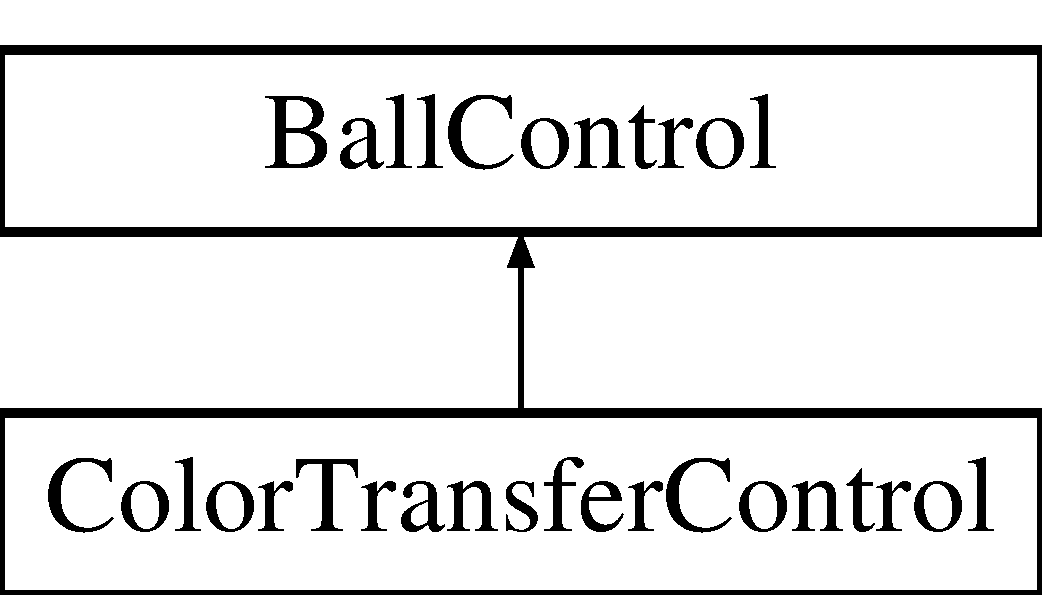
\includegraphics[height=2cm]{classBallControl}
\end{center}
\end{figure}
\subsection*{Public Member Functions}
\begin{DoxyCompactItemize}
\item 
virtual void \hyperlink{classBallControl_af32a9b232b26af69231966ae3aab98d5}{update} (std::vector$<$ \hyperlink{structBall}{Ball} $>$ \&\_\-balls, \hyperlink{classBallGrid}{BallGrid} $\ast$\_\-ballGrid, float \_\-deltaTime, int \_\-maxX, int \_\-maxY)
\begin{DoxyCompactList}\small\item\em update Function intakes the vector of the balls which derives from \hyperlink{structBall}{Ball} class so therefore all values can be set. set mxX and maxY for wall collision detection. \item\end{DoxyCompactList}\item 
void \hyperlink{classBallControl_afa0b3f2735a09bd485ff70ce76ba0ec4}{setGravityDirection} (GravityControl dir)
\begin{DoxyCompactList}\small\item\em setGravityDirection Sets gravity direction control and allows the user to manipulate the direction of the balls \item\end{DoxyCompactList}\item 
virtual void \hyperlink{classBallControl_a1ba25b7c58a9a6ec39ca54daa9e1f488}{mouseDown} (std::vector$<$ \hyperlink{structBall}{Ball} $>$ \&\_\-balls, float \_\-mouseX, float \_\-mouseY)
\begin{DoxyCompactList}\small\item\em mouseDown Takes in the values of the balls so they can be altered depending if the ball is grabbed \item\end{DoxyCompactList}\item 
virtual void \hyperlink{classBallControl_adbc3a6859b147973570a0a531942e595}{mouseUp} (std::vector$<$ \hyperlink{structBall}{Ball} $>$ \&\_\-balls)
\begin{DoxyCompactList}\small\item\em mouseUp takes the values of the balls and apply's them new values when mouse is released \item\end{DoxyCompactList}\item 
virtual void \hyperlink{classBallControl_a18a2fcfe219f8f28319d8f9dcb2bee77}{mouseMotion} (std::vector$<$ \hyperlink{structBall}{Ball} $>$ \&\_\-balls, float \_\-mouseX, float \_\-mouseY)
\begin{DoxyCompactList}\small\item\em mouseMotion takes the general location of the cursor and allows the ball to follow the mouse cursor \item\end{DoxyCompactList}\item 
virtual bool \hyperlink{classBallControl_a85fce07250ce552fd098b6c74d34c588}{mouseBallChecker} (\hyperlink{structBall}{Ball} \&\_\-b, float \_\-mouseX, float \_\-mouseY)
\begin{DoxyCompactList}\small\item\em mouseBallChecker Takes X and Y location for the mouse so it can be located to the location of the ball Also location of the mouse for when the mouse is clicked down \item\end{DoxyCompactList}\item 
virtual void \hyperlink{classBallControl_a352ac9ed1ddedb11892e92ea75e1d171}{updateCollision} (\hyperlink{classBallGrid}{BallGrid} $\ast$\_\-ballGrid)
\begin{DoxyCompactList}\small\item\em updateCollision Takes in the \hyperlink{classBallGrid}{BallGrid} class so the balls can be checked for collision with other balls on the grid \item\end{DoxyCompactList}\item 
virtual void \hyperlink{classBallControl_af84eaea1411dd325db8e94c7adc5d9a3}{collisionChecker} (\hyperlink{structBall}{Ball} $\ast$\_\-ball, std::vector$<$ \hyperlink{structBall}{Ball} $\ast$ $>$ \&\_\-ballsToCheck, int \_\-startingIndex)
\begin{DoxyCompactList}\small\item\em collisionChecker Detects the collision made between a ball and a vector of balls starting at a specific index \item\end{DoxyCompactList}\item 
virtual void \hyperlink{classBallControl_a062a70454845cbf25fe7f15554676ab9}{collisionChecker} (\hyperlink{structBall}{Ball} \&\_\-b1, \hyperlink{structBall}{Ball} \&\_\-b2)
\begin{DoxyCompactList}\small\item\em collisionChecker Detects the collision between two balls in same cell \item\end{DoxyCompactList}\item 
\hypertarget{classBallControl_a6eb0d955ccad645cd5d8865c3bd899a7}{
glm::vec2 \hyperlink{classBallControl_a6eb0d955ccad645cd5d8865c3bd899a7}{getGravityMovement} ()}
\label{classBallControl_a6eb0d955ccad645cd5d8865c3bd899a7}

\begin{DoxyCompactList}\small\item\em vec 2 varible for direction of the gravity movement \item\end{DoxyCompactList}\end{DoxyCompactItemize}
\subsection*{Public Attributes}
\begin{DoxyCompactItemize}
\item 
\hypertarget{classBallControl_ac64a1d833bcd49fa9ab2ebcce3995be6}{
int {\bfseries m\_\-grabbedBall}}
\label{classBallControl_ac64a1d833bcd49fa9ab2ebcce3995be6}

\item 
\hypertarget{classBallControl_a49b276d3d47c744915e289985b54ae4e}{
glm::vec2 {\bfseries m\_\-prevPosition}}
\label{classBallControl_a49b276d3d47c744915e289985b54ae4e}

\item 
\hypertarget{classBallControl_abe4695134fe9cfabef70ed8620de37d2}{
glm::vec2 {\bfseries m\_\-cursorOffset}}
\label{classBallControl_abe4695134fe9cfabef70ed8620de37d2}

\item 
\hypertarget{classBallControl_a64337536a5959b08a7f0b5cb9af52691}{
GravityControl {\bfseries m\_\-gravityControl}}
\label{classBallControl_a64337536a5959b08a7f0b5cb9af52691}

\end{DoxyCompactItemize}


\subsection{Member Function Documentation}
\hypertarget{classBallControl_a062a70454845cbf25fe7f15554676ab9}{
\index{BallControl@{BallControl}!collisionChecker@{collisionChecker}}
\index{collisionChecker@{collisionChecker}!BallControl@{BallControl}}
\subsubsection[{collisionChecker}]{\setlength{\rightskip}{0pt plus 5cm}void BallControl::collisionChecker ({\bf Ball} \& {\em \_\-b1}, \/  {\bf Ball} \& {\em \_\-b2})\hspace{0.3cm}{\ttfamily  \mbox{[}virtual\mbox{]}}}}
\label{classBallControl_a062a70454845cbf25fe7f15554676ab9}


collisionChecker Detects the collision between two balls in same cell 
\begin{DoxyParams}{Parameters}
\item[{\em \_\-b1}]Sets ball one for elastic collision detection \item[{\em \_\-b2}]Sets ball two for elastic collision detection \end{DoxyParams}


Reimplemented in \hyperlink{classColorTransferControl_a9567be01e35663e82691d1756028899a}{ColorTransferControl}.\hypertarget{classBallControl_af84eaea1411dd325db8e94c7adc5d9a3}{
\index{BallControl@{BallControl}!collisionChecker@{collisionChecker}}
\index{collisionChecker@{collisionChecker}!BallControl@{BallControl}}
\subsubsection[{collisionChecker}]{\setlength{\rightskip}{0pt plus 5cm}void BallControl::collisionChecker ({\bf Ball} $\ast$ {\em \_\-ball}, \/  std::vector$<$ {\bf Ball} $\ast$ $>$ \& {\em \_\-ballsToCheck}, \/  int {\em \_\-startingIndex})\hspace{0.3cm}{\ttfamily  \mbox{[}virtual\mbox{]}}}}
\label{classBallControl_af84eaea1411dd325db8e94c7adc5d9a3}


collisionChecker Detects the collision made between a ball and a vector of balls starting at a specific index 
\begin{DoxyParams}{Parameters}
\item[{\em \_\-ball}]Takes the data of balls and check collision in same index \item[{\em \_\-ballsToCheck}]Registers which ball to check in certain cell \item[{\em \_\-startingIndex}]Sets index so ball will check with own cell without duplicating code \end{DoxyParams}


Reimplemented in \hyperlink{classColorTransferControl_a082bba0dbe1e10809d9fb8dc2386a1da}{ColorTransferControl}.\hypertarget{classBallControl_a85fce07250ce552fd098b6c74d34c588}{
\index{BallControl@{BallControl}!mouseBallChecker@{mouseBallChecker}}
\index{mouseBallChecker@{mouseBallChecker}!BallControl@{BallControl}}
\subsubsection[{mouseBallChecker}]{\setlength{\rightskip}{0pt plus 5cm}bool BallControl::mouseBallChecker ({\bf Ball} \& {\em \_\-b}, \/  float {\em \_\-mouseX}, \/  float {\em \_\-mouseY})\hspace{0.3cm}{\ttfamily  \mbox{[}virtual\mbox{]}}}}
\label{classBallControl_a85fce07250ce552fd098b6c74d34c588}


mouseBallChecker Takes X and Y location for the mouse so it can be located to the location of the ball Also location of the mouse for when the mouse is clicked down 
\begin{DoxyParams}{Parameters}
\item[{\em \_\-b}]Set for returning the ball values \item[{\em \_\-mouseX}]Set gets the coordinates of the mouse in X axis \item[{\em \_\-mouseY}]Set gets the coordinates of the mouse in X axis \end{DoxyParams}
\begin{DoxyReturn}{Returns}
The coordinates of the mous linked to ball position 
\end{DoxyReturn}


Reimplemented in \hyperlink{classColorTransferControl_ab4db8c5f585065d55e4beaef3d51b940}{ColorTransferControl}.\hypertarget{classBallControl_a1ba25b7c58a9a6ec39ca54daa9e1f488}{
\index{BallControl@{BallControl}!mouseDown@{mouseDown}}
\index{mouseDown@{mouseDown}!BallControl@{BallControl}}
\subsubsection[{mouseDown}]{\setlength{\rightskip}{0pt plus 5cm}void BallControl::mouseDown (std::vector$<$ {\bf Ball} $>$ \& {\em \_\-balls}, \/  float {\em \_\-mouseX}, \/  float {\em \_\-mouseY})\hspace{0.3cm}{\ttfamily  \mbox{[}virtual\mbox{]}}}}
\label{classBallControl_a1ba25b7c58a9a6ec39ca54daa9e1f488}


mouseDown Takes in the values of the balls so they can be altered depending if the ball is grabbed 
\begin{DoxyParams}{Parameters}
\item[{\em \_\-balls}]Applys the data of balls for when the mouse is down \item[{\em \_\-mouseX}]Takes coordinates of the mouse in x axis \item[{\em \_\-mouseY}]Takes coordinates of the mouse in Y axis \end{DoxyParams}


Reimplemented in \hyperlink{classColorTransferControl_ac0acd46f1620035c8d7a830206fce6b8}{ColorTransferControl}.\hypertarget{classBallControl_a18a2fcfe219f8f28319d8f9dcb2bee77}{
\index{BallControl@{BallControl}!mouseMotion@{mouseMotion}}
\index{mouseMotion@{mouseMotion}!BallControl@{BallControl}}
\subsubsection[{mouseMotion}]{\setlength{\rightskip}{0pt plus 5cm}void BallControl::mouseMotion (std::vector$<$ {\bf Ball} $>$ \& {\em \_\-balls}, \/  float {\em \_\-mouseX}, \/  float {\em \_\-mouseY})\hspace{0.3cm}{\ttfamily  \mbox{[}virtual\mbox{]}}}}
\label{classBallControl_a18a2fcfe219f8f28319d8f9dcb2bee77}


mouseMotion takes the general location of the cursor and allows the ball to follow the mouse cursor 
\begin{DoxyParams}{Parameters}
\item[{\em \_\-balls}]Sets the ball and allows it to be affected by the mosue \item[{\em \_\-mouseX}]Gets the coordinates of the mouse in x axis \item[{\em \_\-mouseY}]Gets the coordinates of the mouse in y axis \end{DoxyParams}


Reimplemented in \hyperlink{classColorTransferControl_a84567646b6a7d814aa8de8660da69543}{ColorTransferControl}.\hypertarget{classBallControl_adbc3a6859b147973570a0a531942e595}{
\index{BallControl@{BallControl}!mouseUp@{mouseUp}}
\index{mouseUp@{mouseUp}!BallControl@{BallControl}}
\subsubsection[{mouseUp}]{\setlength{\rightskip}{0pt plus 5cm}void BallControl::mouseUp (std::vector$<$ {\bf Ball} $>$ \& {\em \_\-balls})\hspace{0.3cm}{\ttfamily  \mbox{[}virtual\mbox{]}}}}
\label{classBallControl_adbc3a6859b147973570a0a531942e595}


mouseUp takes the values of the balls and apply's them new values when mouse is released 
\begin{DoxyParams}{Parameters}
\item[{\em \_\-balls}]Takes the data of balls and applys it to mouse up \end{DoxyParams}


Reimplemented in \hyperlink{classColorTransferControl_a335ef9511d0cacec325a154c106bb1da}{ColorTransferControl}.\hypertarget{classBallControl_afa0b3f2735a09bd485ff70ce76ba0ec4}{
\index{BallControl@{BallControl}!setGravityDirection@{setGravityDirection}}
\index{setGravityDirection@{setGravityDirection}!BallControl@{BallControl}}
\subsubsection[{setGravityDirection}]{\setlength{\rightskip}{0pt plus 5cm}void BallControl::setGravityDirection (GravityControl {\em dir})\hspace{0.3cm}{\ttfamily  \mbox{[}inline\mbox{]}}}}
\label{classBallControl_afa0b3f2735a09bd485ff70ce76ba0ec4}


setGravityDirection Sets gravity direction control and allows the user to manipulate the direction of the balls 
\begin{DoxyParams}{Parameters}
\item[{\em dir}]sets direction of the ball \end{DoxyParams}
\hypertarget{classBallControl_af32a9b232b26af69231966ae3aab98d5}{
\index{BallControl@{BallControl}!update@{update}}
\index{update@{update}!BallControl@{BallControl}}
\subsubsection[{update}]{\setlength{\rightskip}{0pt plus 5cm}void BallControl::update (std::vector$<$ {\bf Ball} $>$ \& {\em \_\-balls}, \/  {\bf BallGrid} $\ast$ {\em \_\-ballGrid}, \/  float {\em \_\-deltaTime}, \/  int {\em \_\-maxX}, \/  int {\em \_\-maxY})\hspace{0.3cm}{\ttfamily  \mbox{[}virtual\mbox{]}}}}
\label{classBallControl_af32a9b232b26af69231966ae3aab98d5}


update Function intakes the vector of the balls which derives from \hyperlink{structBall}{Ball} class so therefore all values can be set. set mxX and maxY for wall collision detection. 
\begin{DoxyParams}{Parameters}
\item[{\em \_\-balls}]\item[{\em \_\-ballGrid}]\hyperlink{classBallGrid}{BallGrid} to allow the input of the 2D grid to update each ball with spatial partitioning \item[{\em \_\-deltaTime}]DeltaTime is set to keep motion at a fix rate \item[{\em \_\-maxX}]Set for wall collision in X direction \item[{\em \_\-maxY}]Set for wall collision in Y direction \end{DoxyParams}


Reimplemented in \hyperlink{classColorTransferControl_add37c8ee8e911a13ecec98cf09fc81c4}{ColorTransferControl}.\hypertarget{classBallControl_a352ac9ed1ddedb11892e92ea75e1d171}{
\index{BallControl@{BallControl}!updateCollision@{updateCollision}}
\index{updateCollision@{updateCollision}!BallControl@{BallControl}}
\subsubsection[{updateCollision}]{\setlength{\rightskip}{0pt plus 5cm}void BallControl::updateCollision ({\bf BallGrid} $\ast$ {\em \_\-ballGrid})\hspace{0.3cm}{\ttfamily  \mbox{[}virtual\mbox{]}}}}
\label{classBallControl_a352ac9ed1ddedb11892e92ea75e1d171}


updateCollision Takes in the \hyperlink{classBallGrid}{BallGrid} class so the balls can be checked for collision with other balls on the grid 
\begin{DoxyParams}{Parameters}
\item[{\em \_\-ballGrid}]Checks the ballGrid to update collision \end{DoxyParams}


Reimplemented in \hyperlink{classColorTransferControl_a9f54f20a18940cf66c08a994eb8dfb01}{ColorTransferControl}.

The documentation for this class was generated from the following files:\begin{DoxyCompactItemize}
\item 
Include/BallGame/\hyperlink{BallControl_8h}{BallControl.h}\item 
src/Uni/\hyperlink{BallControl_8cpp}{BallControl.cpp}\end{DoxyCompactItemize}

\hypertarget{classBallGrid}{
\section{BallGrid Class Reference}
\label{classBallGrid}\index{BallGrid@{BallGrid}}
}


{\ttfamily \#include $<$BallGrid.h$>$}\subsection*{Public Member Functions}
\begin{DoxyCompactItemize}
\item 
\hypertarget{classBallGrid_acdcc4d6951173ed948f47f0dcb929ff9}{
{\bfseries BallGrid} (int width, int height, int cellSize)}
\label{classBallGrid_acdcc4d6951173ed948f47f0dcb929ff9}

\item 
\hypertarget{classBallGrid_a4fc613f1cf978f3e67c4a8bbf4d6f9a8}{
\hyperlink{structCell}{Cell} $\ast$ \hyperlink{classBallGrid_a4fc613f1cf978f3e67c4a8bbf4d6f9a8}{getCell} (int x, int y)}
\label{classBallGrid_a4fc613f1cf978f3e67c4a8bbf4d6f9a8}

\begin{DoxyCompactList}\small\item\em Here I overload the getCell function as each one performs a similar job. \item\end{DoxyCompactList}\item 
\hyperlink{structCell}{Cell} $\ast$ \hyperlink{classBallGrid_a1c1b46810cee5738bc9cdcc98132f37e}{getCell} (const glm::vec2 \&pos)
\begin{DoxyCompactList}\small\item\em get cell based on position of the cell in the window \item\end{DoxyCompactList}\item 
void \hyperlink{classBallGrid_ad3a834b61100b1ca532c47c8b3b68062}{addBall} (\hyperlink{structBall}{Ball} $\ast$ball)
\begin{DoxyCompactList}\small\item\em adds a ball and determines what cell it belongs to \item\end{DoxyCompactList}\item 
void \hyperlink{classBallGrid_a1ee46472584ce1515e22d3a8b5c4f531}{addBall} (\hyperlink{structBall}{Ball} $\ast$ball, \hyperlink{structCell}{Cell} $\ast$cell)
\begin{DoxyCompactList}\small\item\em adds ball to specific cell \item\end{DoxyCompactList}\item 
void \hyperlink{classBallGrid_a468ea1f13fb2e2860e2d393a199a6116}{removeBall} (\hyperlink{structBall}{Ball} $\ast$ball)
\begin{DoxyCompactList}\small\item\em Removes the ball from the grid. \item\end{DoxyCompactList}\end{DoxyCompactItemize}
\subsection*{Public Attributes}
\begin{DoxyCompactItemize}
\item 
\hypertarget{classBallGrid_a1784f4acd2d7dda8cf47b52ff9869416}{
std::vector$<$ \hyperlink{structCell}{Cell} $>$ {\bfseries m\_\-cells}}
\label{classBallGrid_a1784f4acd2d7dda8cf47b52ff9869416}

\item 
\hypertarget{classBallGrid_a27151691c66dab33adb36622089294c0}{
int {\bfseries m\_\-cellSize}}
\label{classBallGrid_a27151691c66dab33adb36622089294c0}

\item 
\hypertarget{classBallGrid_a0b9fc1fe2f4465113fcf968523a7f8ae}{
int {\bfseries m\_\-width}}
\label{classBallGrid_a0b9fc1fe2f4465113fcf968523a7f8ae}

\item 
\hypertarget{classBallGrid_ada7cfe8e209b93cca5329b048b1dc0a3}{
int {\bfseries m\_\-height}}
\label{classBallGrid_ada7cfe8e209b93cca5329b048b1dc0a3}

\item 
\hypertarget{classBallGrid_afa477104004a39645546c48c8fe891b6}{
int {\bfseries m\_\-numCellsX}}
\label{classBallGrid_afa477104004a39645546c48c8fe891b6}

\item 
\hypertarget{classBallGrid_a47e202910b6408d75837fa8f9e99e82a}{
int {\bfseries m\_\-numCellsY}}
\label{classBallGrid_a47e202910b6408d75837fa8f9e99e82a}

\end{DoxyCompactItemize}
\subsection*{Friends}
\begin{DoxyCompactItemize}
\item 
\hypertarget{classBallGrid_a96c3892ebe4274ff47fade92c0bf313f}{
class \hyperlink{classBallGrid_a96c3892ebe4274ff47fade92c0bf313f}{BallControl}}
\label{classBallGrid_a96c3892ebe4274ff47fade92c0bf313f}

\end{DoxyCompactItemize}


\subsection{Detailed Description}
Has a number of balls which will be stored in cells To accomplish this I used a 2D grid of cells 

\subsection{Member Function Documentation}
\hypertarget{classBallGrid_a1ee46472584ce1515e22d3a8b5c4f531}{
\index{BallGrid@{BallGrid}!addBall@{addBall}}
\index{addBall@{addBall}!BallGrid@{BallGrid}}
\subsubsection[{addBall}]{\setlength{\rightskip}{0pt plus 5cm}void BallGrid::addBall ({\bf Ball} $\ast$ {\em ball}, \/  {\bf Cell} $\ast$ {\em cell})}}
\label{classBallGrid_a1ee46472584ce1515e22d3a8b5c4f531}


adds ball to specific cell 
\begin{DoxyParams}{Parameters}
\item[{\em ball}]\item[{\em cell}]\end{DoxyParams}
\hypertarget{classBallGrid_ad3a834b61100b1ca532c47c8b3b68062}{
\index{BallGrid@{BallGrid}!addBall@{addBall}}
\index{addBall@{addBall}!BallGrid@{BallGrid}}
\subsubsection[{addBall}]{\setlength{\rightskip}{0pt plus 5cm}void BallGrid::addBall ({\bf Ball} $\ast$ {\em ball})}}
\label{classBallGrid_ad3a834b61100b1ca532c47c8b3b68062}


adds a ball and determines what cell it belongs to 
\begin{DoxyParams}{Parameters}
\item[{\em ball}]\end{DoxyParams}
\hypertarget{classBallGrid_a1c1b46810cee5738bc9cdcc98132f37e}{
\index{BallGrid@{BallGrid}!getCell@{getCell}}
\index{getCell@{getCell}!BallGrid@{BallGrid}}
\subsubsection[{getCell}]{\setlength{\rightskip}{0pt plus 5cm}{\bf Cell} $\ast$ BallGrid::getCell (const glm::vec2 \& {\em pos})}}
\label{classBallGrid_a1c1b46810cee5738bc9cdcc98132f37e}


get cell based on position of the cell in the window 
\begin{DoxyParams}{Parameters}
\item[{\em pos}]\end{DoxyParams}
\begin{DoxyReturn}{Returns}

\end{DoxyReturn}
\hypertarget{classBallGrid_a468ea1f13fb2e2860e2d393a199a6116}{
\index{BallGrid@{BallGrid}!removeBall@{removeBall}}
\index{removeBall@{removeBall}!BallGrid@{BallGrid}}
\subsubsection[{removeBall}]{\setlength{\rightskip}{0pt plus 5cm}void BallGrid::removeBall ({\bf Ball} $\ast$ {\em ball})}}
\label{classBallGrid_a468ea1f13fb2e2860e2d393a199a6116}


Removes the ball from the grid. remove the ball from the cell 

The documentation for this class was generated from the following files:\begin{DoxyCompactItemize}
\item 
Include/BallGame/\hyperlink{BallGrid_8h}{BallGrid.h}\item 
src/Uni/\hyperlink{BallGrid_8cpp}{BallGrid.cpp}\end{DoxyCompactItemize}

\hypertarget{classBallRenderer}{
\section{BallRenderer Class Reference}
\label{classBallRenderer}\index{BallRenderer@{BallRenderer}}
}
Inheritance diagram for BallRenderer::\begin{figure}[H]
\begin{center}
\leavevmode
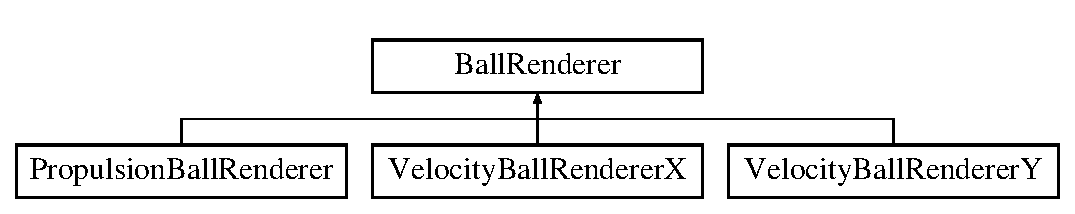
\includegraphics[height=2cm]{classBallRenderer}
\end{center}
\end{figure}
\subsection*{Public Member Functions}
\begin{DoxyCompactItemize}
\item 
void \hyperlink{classBallRenderer_a6340a67dc1f573c71ea9934f35560256}{initShaders} ()
\item 
virtual void \hyperlink{classBallRenderer_a6169ba2a00e8d15fde87a3ee4552cf66}{renderBalls} (\hyperlink{classRandini_1_1SpriteLoader}{Randini::SpriteLoader} \&spriteLoader, const std::vector$<$ \hyperlink{structBall}{Ball} $>$ \&balls, const glm::mat4 \&projectionMatrix)
\end{DoxyCompactItemize}
\subsection*{Protected Attributes}
\begin{DoxyCompactItemize}
\item 
\hypertarget{classBallRenderer_a3e9fad7afb392a4be134536bbb4a209a}{
std::unique\_\-ptr$<$ \hyperlink{classRandini_1_1GLSLProgram}{Randini::GLSLProgram} $>$ {\bfseries m\_\-program}}
\label{classBallRenderer_a3e9fad7afb392a4be134536bbb4a209a}

\end{DoxyCompactItemize}


\subsection{Member Function Documentation}
\hypertarget{classBallRenderer_a6340a67dc1f573c71ea9934f35560256}{
\index{BallRenderer@{BallRenderer}!initShaders@{initShaders}}
\index{initShaders@{initShaders}!BallRenderer@{BallRenderer}}
\subsubsection[{initShaders}]{\setlength{\rightskip}{0pt plus 5cm}void BallRenderer::initShaders ()}}
\label{classBallRenderer_a6340a67dc1f573c71ea9934f35560256}
As soon as the program calls render balls with a program whihc is null it will allocate a new one Inits all shaders from GLSL shader located in Randini Engine Adds the attributes and links the shaders \hypertarget{classBallRenderer_a6169ba2a00e8d15fde87a3ee4552cf66}{
\index{BallRenderer@{BallRenderer}!renderBalls@{renderBalls}}
\index{renderBalls@{renderBalls}!BallRenderer@{BallRenderer}}
\subsubsection[{renderBalls}]{\setlength{\rightskip}{0pt plus 5cm}void BallRenderer::renderBalls ({\bf Randini::SpriteLoader} \& {\em spriteLoader}, \/  const std::vector$<$ {\bf Ball} $>$ \& {\em balls}, \/  const glm::mat4 \& {\em projectionMatrix})\hspace{0.3cm}{\ttfamily  \mbox{[}virtual\mbox{]}}}}
\label{classBallRenderer_a6169ba2a00e8d15fde87a3ee4552cf66}
Make this a virtual function as I want to derive form this Imports the sprites from the game engine renders a list of balls to render all the balls Instead of rendering a single ball loop through all the balls 

Reimplemented in \hyperlink{classPropulsionBallRenderer_a9ebdecb973a1a399b4699d7e5c47c0b9}{PropulsionBallRenderer}, \hyperlink{classVelocityBallRendererX_ad0ef24ce7ba5116231f4a47aff280f12}{VelocityBallRendererX}, and \hyperlink{classVelocityBallRendererY_aee5499c81382f071f58467d2040e36c9}{VelocityBallRendererY}.

The documentation for this class was generated from the following files:\begin{DoxyCompactItemize}
\item 
Include/BallGame/\hyperlink{BallRenderer_8h}{BallRenderer.h}\item 
src/Uni/\hyperlink{BallRenderer_8cpp}{BallRenderer.cpp}\end{DoxyCompactItemize}

\hypertarget{structBallSpawnSystem}{
\section{BallSpawnSystem Struct Reference}
\label{structBallSpawnSystem}\index{BallSpawnSystem@{BallSpawnSystem}}
}
\subsection*{Public Member Functions}
\begin{DoxyCompactItemize}
\item 
\hypertarget{structBallSpawnSystem_a1123b7053659b1ae8aa6cdd2981b0c01}{
{\bfseries BallSpawnSystem} (const \hyperlink{structRandini_1_1ColorRGBA8}{Randini::ColorRGBA8} \&color, float m\_\-radius, float mass, float minSpeed, float maxSpeed, float prob)}
\label{structBallSpawnSystem_a1123b7053659b1ae8aa6cdd2981b0c01}

\end{DoxyCompactItemize}
\subsection*{Public Attributes}
\begin{DoxyCompactItemize}
\item 
\hypertarget{structBallSpawnSystem_a3bb75a1b6cf6aac33081119dd2198777}{
\hyperlink{structRandini_1_1ColorRGBA8}{Randini::ColorRGBA8} {\bfseries color}}
\label{structBallSpawnSystem_a3bb75a1b6cf6aac33081119dd2198777}

\item 
\hypertarget{structBallSpawnSystem_a7f9ac4289317532de48df707153e1bd5}{
float {\bfseries m\_\-radius}}
\label{structBallSpawnSystem_a7f9ac4289317532de48df707153e1bd5}

\item 
\hypertarget{structBallSpawnSystem_ad718e14c232b6006f0722d89ed591107}{
float {\bfseries mass}}
\label{structBallSpawnSystem_ad718e14c232b6006f0722d89ed591107}

\item 
\hypertarget{structBallSpawnSystem_afcdf95906eddebf9fc5324ba664959e1}{
float {\bfseries probability}}
\label{structBallSpawnSystem_afcdf95906eddebf9fc5324ba664959e1}

\item 
\hypertarget{structBallSpawnSystem_a1176dfb472047938d78177daceb3b9b8}{
\hyperlink{MainGame_8h_a3bbd6868c609bd755d6336c79fad44aa}{RandomDistribution} {\bfseries randSpeed}}
\label{structBallSpawnSystem_a1176dfb472047938d78177daceb3b9b8}

\end{DoxyCompactItemize}


The documentation for this struct was generated from the following file:\begin{DoxyCompactItemize}
\item 
src/Uni/\hyperlink{MainGame_8cpp}{MainGame.cpp}\end{DoxyCompactItemize}

\hypertarget{classRandini_1_1Camera2D}{
\section{Randini::Camera2D Class Reference}
\label{classRandini_1_1Camera2D}\index{Randini::Camera2D@{Randini::Camera2D}}
}
\subsection*{Public Member Functions}
\begin{DoxyCompactItemize}
\item 
\hypertarget{classRandini_1_1Camera2D_ab658d7f26ed3fec10ac4e16882ea85e0}{
void {\bfseries init} (int \_\-screenWidth, int \_\-screenHeight)}
\label{classRandini_1_1Camera2D_ab658d7f26ed3fec10ac4e16882ea85e0}

\item 
\hypertarget{classRandini_1_1Camera2D_a6624d7fd91cdf68e305568aa2ace5539}{
void {\bfseries updateCamera} ()}
\label{classRandini_1_1Camera2D_a6624d7fd91cdf68e305568aa2ace5539}

\item 
\hypertarget{classRandini_1_1Camera2D_a545b5ce7ca9f2c99b8fc7837d6ee4872}{
glm::vec2 {\bfseries getWorldScreenCoords} (glm::vec2 screenCoords)}
\label{classRandini_1_1Camera2D_a545b5ce7ca9f2c99b8fc7837d6ee4872}

\item 
\hypertarget{classRandini_1_1Camera2D_a13745cf68d6dc73d6759b3a3ee1c4cb1}{
void {\bfseries setPosition} (const glm::vec2 \&newPosition)}
\label{classRandini_1_1Camera2D_a13745cf68d6dc73d6759b3a3ee1c4cb1}

\item 
\hypertarget{classRandini_1_1Camera2D_ad9bb40c09c7f51960574a795124bf1ad}{
glm::vec2 {\bfseries getPosition} ()}
\label{classRandini_1_1Camera2D_ad9bb40c09c7f51960574a795124bf1ad}

\item 
\hypertarget{classRandini_1_1Camera2D_a6446d430b1c5b5c3f3435c5ebc8fdfa6}{
void {\bfseries setScale} (float newScale)}
\label{classRandini_1_1Camera2D_a6446d430b1c5b5c3f3435c5ebc8fdfa6}

\item 
\hypertarget{classRandini_1_1Camera2D_a6e5515a9d361baef52afc11deba94426}{
float {\bfseries getScale} ()}
\label{classRandini_1_1Camera2D_a6e5515a9d361baef52afc11deba94426}

\item 
\hypertarget{classRandini_1_1Camera2D_adac18a3635569b0868c5d77e8f8635a8}{
glm::mat4 {\bfseries getCameraMatrix} ()}
\label{classRandini_1_1Camera2D_adac18a3635569b0868c5d77e8f8635a8}

\end{DoxyCompactItemize}


The documentation for this class was generated from the following files:\begin{DoxyCompactItemize}
\item 
Include/Randini/\hyperlink{Camera2D_8h}{Camera2D.h}\item 
src/Randini/\hyperlink{Camera2D_8cpp}{Camera2D.cpp}\end{DoxyCompactItemize}

\hypertarget{structCell}{
\section{Cell Struct Reference}
\label{structCell}\index{Cell@{Cell}}
}


Inlcude vector as using vector for the list.  


{\ttfamily \#include $<$BallGrid.h$>$}\subsection*{Public Attributes}
\begin{DoxyCompactItemize}
\item 
\hypertarget{structCell_a69885480f0ba645aa3e9c35d1b0580c3}{
std::vector$<$ \hyperlink{structBall}{Ball} $\ast$ $>$ {\bfseries balls}}
\label{structCell_a69885480f0ba645aa3e9c35d1b0580c3}

\end{DoxyCompactItemize}


\subsection{Detailed Description}
Inlcude vector as using vector for the list. This struct contains a list of balls Made a struct over class as it contains no methods and is fairly simple 

The documentation for this struct was generated from the following file:\begin{DoxyCompactItemize}
\item 
Include/BallGame/\hyperlink{BallGrid_8h}{BallGrid.h}\end{DoxyCompactItemize}

\hypertarget{structRandini_1_1ColorRGBA8}{
\section{Randini::ColorRGBA8 Struct Reference}
\label{structRandini_1_1ColorRGBA8}\index{Randini::ColorRGBA8@{Randini::ColorRGBA8}}
}
\subsection*{Public Member Functions}
\begin{DoxyCompactItemize}
\item 
\hypertarget{structRandini_1_1ColorRGBA8_a396717be022d8a9aedaebcce68380c55}{
{\bfseries ColorRGBA8} (GLubyte R, GLubyte G, GLubyte B, GLubyte A)}
\label{structRandini_1_1ColorRGBA8_a396717be022d8a9aedaebcce68380c55}

\end{DoxyCompactItemize}
\subsection*{Public Attributes}
\begin{DoxyCompactItemize}
\item 
\hypertarget{structRandini_1_1ColorRGBA8_a699de73c4f40c7acc194e192adbc3f3c}{
GLubyte {\bfseries r}}
\label{structRandini_1_1ColorRGBA8_a699de73c4f40c7acc194e192adbc3f3c}

\item 
\hypertarget{structRandini_1_1ColorRGBA8_abaacd81b0deea181df45daf4f0a2ebf5}{
GLubyte {\bfseries g}}
\label{structRandini_1_1ColorRGBA8_abaacd81b0deea181df45daf4f0a2ebf5}

\item 
\hypertarget{structRandini_1_1ColorRGBA8_af84fd1ca49952f1d59d03f658d7b2ba5}{
GLubyte {\bfseries b}}
\label{structRandini_1_1ColorRGBA8_af84fd1ca49952f1d59d03f658d7b2ba5}

\item 
\hypertarget{structRandini_1_1ColorRGBA8_a0eed6101efaa81166984a78c08b02ed4}{
GLubyte {\bfseries a}}
\label{structRandini_1_1ColorRGBA8_a0eed6101efaa81166984a78c08b02ed4}

\end{DoxyCompactItemize}


The documentation for this struct was generated from the following file:\begin{DoxyCompactItemize}
\item 
Include/Randini/\hyperlink{Vertex_8h}{Vertex.h}\end{DoxyCompactItemize}

\hypertarget{classColorTransferControl}{
\section{ColorTransferControl Class Reference}
\label{classColorTransferControl}\index{ColorTransferControl@{ColorTransferControl}}
}
Inheritance diagram for ColorTransferControl::\begin{figure}[H]
\begin{center}
\leavevmode
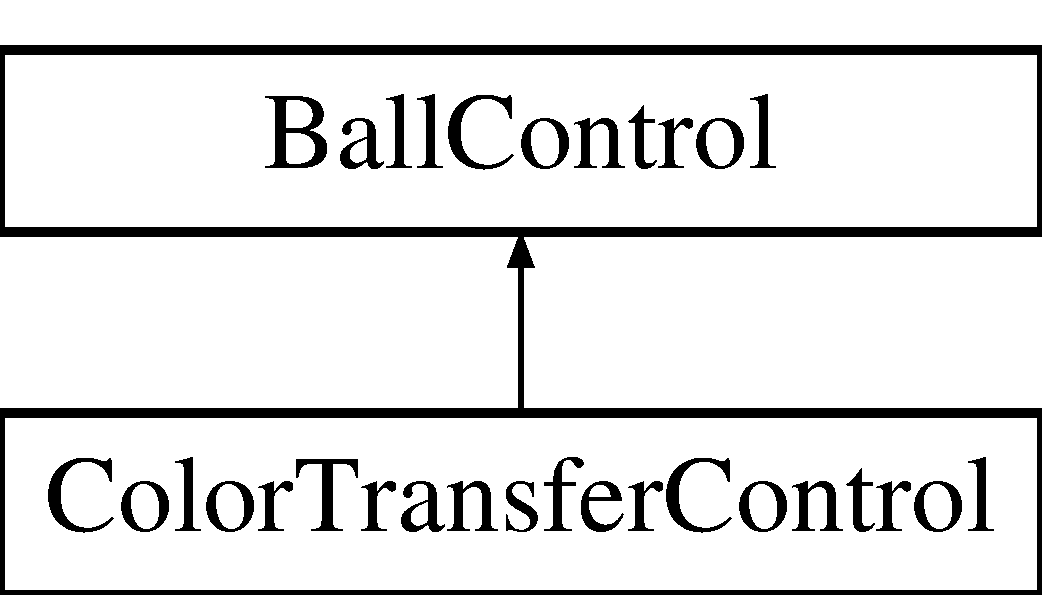
\includegraphics[height=2cm]{classColorTransferControl}
\end{center}
\end{figure}
\subsection*{Public Member Functions}
\begin{DoxyCompactItemize}
\item 
\hypertarget{classColorTransferControl_a446d087e090cb13cefdffb89e8c409e3}{
glm::vec2 \hyperlink{classColorTransferControl_a446d087e090cb13cefdffb89e8c409e3}{getGravityMovement} ()}
\label{classColorTransferControl_a446d087e090cb13cefdffb89e8c409e3}

\begin{DoxyCompactList}\small\item\em vec 2 varible for direction of the gravity movement \item\end{DoxyCompactList}\item 
virtual bool \hyperlink{classColorTransferControl_a9bce863f9d08a2dd596a56a432861559}{mouseBallChecker} (\hyperlink{structBall}{Ball} \&b, float mouseX, float mouseY)
\item 
\hypertarget{classColorTransferControl_abac3a089bfe8d05916392cd7dd6807e3}{
virtual void {\bfseries mouseDown} (std::vector$<$ \hyperlink{structBall}{Ball} $>$ \&balls, float mouseX, float mouseY)}
\label{classColorTransferControl_abac3a089bfe8d05916392cd7dd6807e3}

\item 
\hypertarget{classColorTransferControl_a84e96588725965ae2e92b35c22f4a629}{
virtual void {\bfseries mouseUp} (std::vector$<$ \hyperlink{structBall}{Ball} $>$ \&balls)}
\label{classColorTransferControl_a84e96588725965ae2e92b35c22f4a629}

\item 
\hypertarget{classColorTransferControl_a77c38be1e1f33b81f1c4a3f82d671623}{
virtual void {\bfseries mouseMotion} (std::vector$<$ \hyperlink{structBall}{Ball} $>$ \&balls, float mouseX, float mouseY)}
\label{classColorTransferControl_a77c38be1e1f33b81f1c4a3f82d671623}

\item 
virtual void \hyperlink{classColorTransferControl_acbe9581f0be7624c9bc33d40e2ee1a6b}{update} (std::vector$<$ \hyperlink{structBall}{Ball} $>$ \&balls, \hyperlink{classBallGrid}{BallGrid} $\ast$ballGrid, float deltaTime, int maxX, int maxY)
\item 
\hypertarget{classColorTransferControl_aa8608d2417309f4d3a09e1b613060249}{
virtual void {\bfseries updateCollision} (\hyperlink{classBallGrid}{BallGrid} $\ast$ballGrid)}
\label{classColorTransferControl_aa8608d2417309f4d3a09e1b613060249}

\item 
\hypertarget{classColorTransferControl_a2a5fae5e92692b533d92ddf112661a17}{
virtual void {\bfseries collisionChecker} (\hyperlink{structBall}{Ball} $\ast$ball, std::vector$<$ \hyperlink{structBall}{Ball} $\ast$ $>$ \&ballsToCheck, int startingIndex)}
\label{classColorTransferControl_a2a5fae5e92692b533d92ddf112661a17}

\item 
\hypertarget{classColorTransferControl_a3071e883130aabc2b0642a75bf9225dc}{
virtual void {\bfseries collisionChecker} (\hyperlink{structBall}{Ball} \&b1, \hyperlink{structBall}{Ball} \&b2)}
\label{classColorTransferControl_a3071e883130aabc2b0642a75bf9225dc}

\end{DoxyCompactItemize}


\subsection{Member Function Documentation}
\hypertarget{classColorTransferControl_a9bce863f9d08a2dd596a56a432861559}{
\index{ColorTransferControl@{ColorTransferControl}!mouseBallChecker@{mouseBallChecker}}
\index{mouseBallChecker@{mouseBallChecker}!ColorTransferControl@{ColorTransferControl}}
\subsubsection[{mouseBallChecker}]{\setlength{\rightskip}{0pt plus 5cm}bool ColorTransferControl::mouseBallChecker ({\bf Ball} \& {\em b}, \/  float {\em mouseX}, \/  float {\em mouseY})\hspace{0.3cm}{\ttfamily  \mbox{[}virtual\mbox{]}}}}
\label{classColorTransferControl_a9bce863f9d08a2dd596a56a432861559}
MouseBallChecker: Takes X and Y location for the mouse so it can be located to the location of the ball /// MouseDown: Takes in the values of the balls so they can be altered depending if the ball is grabbed /// Also location of the mouse for when the mouse is clicked down /// MouseUP: Takes the values of the balls and apply's them new values when mouse is released /// MouseMotion: Takes the general location of the cursor and allows the ball to follow the mouse cursor /// UpdateCollision: Takes in the \hyperlink{classBallGrid}{BallGrid} class so the balls can be checked for collision with other balls on the grid /// CollisisonChecker: Detects the collision made between a ball and a vector of balls starting at a specific index /// 

Reimplemented from \hyperlink{classBallControl_a4f811993f5e8988eb4f4ab3c03dadf52}{BallControl}.\hypertarget{classColorTransferControl_acbe9581f0be7624c9bc33d40e2ee1a6b}{
\index{ColorTransferControl@{ColorTransferControl}!update@{update}}
\index{update@{update}!ColorTransferControl@{ColorTransferControl}}
\subsubsection[{update}]{\setlength{\rightskip}{0pt plus 5cm}void ColorTransferControl::update (std::vector$<$ {\bf Ball} $>$ \& {\em \_\-balls}, \/  {\bf BallGrid} $\ast$ {\em \_\-ballGrid}, \/  float {\em \_\-deltaTime}, \/  int {\em \_\-maxX}, \/  int {\em \_\-maxY})\hspace{0.3cm}{\ttfamily  \mbox{[}virtual\mbox{]}}}}
\label{classColorTransferControl_acbe9581f0be7624c9bc33d40e2ee1a6b}
Function intakes the vector of the balls which derives from \hyperlink{structBall}{Ball} class so therefore all values can be set. \hyperlink{classBallGrid}{BallGrid} to allow the input of the 2D grid to update each ball with spatial partitioning Delta time as all function need to be set to deltaTime, set mxX and maxY for wall collision detection. 

Reimplemented from \hyperlink{classBallControl_af32a9b232b26af69231966ae3aab98d5}{BallControl}.

The documentation for this class was generated from the following files:\begin{DoxyCompactItemize}
\item 
Include/BallGame/\hyperlink{BallControl_8h}{BallControl.h}\item 
src/Uni/\hyperlink{BallControl_8cpp}{BallControl.cpp}\end{DoxyCompactItemize}

\hypertarget{classRandini_1_1FPSLimiter}{
\section{Randini::FPSLimiter Class Reference}
\label{classRandini_1_1FPSLimiter}\index{Randini::FPSLimiter@{Randini::FPSLimiter}}
}
\subsection*{Public Member Functions}
\begin{DoxyCompactItemize}
\item 
\hypertarget{classRandini_1_1FPSLimiter_a3024a959139c6a9b2d2c583200d69a0c}{
void {\bfseries init} (float maxFPS)}
\label{classRandini_1_1FPSLimiter_a3024a959139c6a9b2d2c583200d69a0c}

\item 
\hypertarget{classRandini_1_1FPSLimiter_ab791c46a558dc4f7dfca408f92563bf5}{
void {\bfseries setMaxFPS} (float maxFPS)}
\label{classRandini_1_1FPSLimiter_ab791c46a558dc4f7dfca408f92563bf5}

\item 
\hypertarget{classRandini_1_1FPSLimiter_ab3c41c74d451ebdcba9f448fd60efeaa}{
void {\bfseries begin} ()}
\label{classRandini_1_1FPSLimiter_ab3c41c74d451ebdcba9f448fd60efeaa}

\item 
\hypertarget{classRandini_1_1FPSLimiter_adde6384240089bf3e87ce5d5dc114c60}{
float {\bfseries end} ()}
\label{classRandini_1_1FPSLimiter_adde6384240089bf3e87ce5d5dc114c60}

\end{DoxyCompactItemize}


The documentation for this class was generated from the following files:\begin{DoxyCompactItemize}
\item 
Include/Randini/\hyperlink{Timer_8h}{Timer.h}\item 
src/Randini/\hyperlink{Timer_8cpp}{Timer.cpp}\end{DoxyCompactItemize}

\hypertarget{classRandini_1_1GLSLProgram}{
\section{Randini::GLSLProgram Class Reference}
\label{classRandini_1_1GLSLProgram}\index{Randini::GLSLProgram@{Randini::GLSLProgram}}
}
\subsection*{Public Member Functions}
\begin{DoxyCompactItemize}
\item 
\hypertarget{classRandini_1_1GLSLProgram_a73328c415caa63862b713bb840b85532}{
void {\bfseries compileShaders} (const std::string \&vertexShaderFilePath, const std::string \&fragmentShaderFilePath)}
\label{classRandini_1_1GLSLProgram_a73328c415caa63862b713bb840b85532}

\item 
\hypertarget{classRandini_1_1GLSLProgram_aa67b3edb1c8eae84dc65d5e913e144cd}{
void {\bfseries linkShader} ()}
\label{classRandini_1_1GLSLProgram_aa67b3edb1c8eae84dc65d5e913e144cd}

\item 
\hypertarget{classRandini_1_1GLSLProgram_ad623f8c42dfa974c7820949905a53d18}{
void {\bfseries addAttribute} (const std::string \&attributeName)}
\label{classRandini_1_1GLSLProgram_ad623f8c42dfa974c7820949905a53d18}

\item 
\hypertarget{classRandini_1_1GLSLProgram_a8ed1430de4e2629d6dcddf8eafd6ce09}{
GLint {\bfseries getUniformLocation} (const std::string \&uniformName)}
\label{classRandini_1_1GLSLProgram_a8ed1430de4e2629d6dcddf8eafd6ce09}

\item 
\hypertarget{classRandini_1_1GLSLProgram_a7371ee6e41ba0d03a61663d67551da48}{
void {\bfseries use} ()}
\label{classRandini_1_1GLSLProgram_a7371ee6e41ba0d03a61663d67551da48}

\item 
\hypertarget{classRandini_1_1GLSLProgram_a29fb698f73e40621ec181ed7c3c3e7be}{
void {\bfseries unuse} ()}
\label{classRandini_1_1GLSLProgram_a29fb698f73e40621ec181ed7c3c3e7be}

\end{DoxyCompactItemize}


The documentation for this class was generated from the following files:\begin{DoxyCompactItemize}
\item 
Include/Randini/\hyperlink{GLSLProgram_8h}{GLSLProgram.h}\item 
src/Randini/\hyperlink{GLSLProgram_8cpp}{GLSLProgram.cpp}\end{DoxyCompactItemize}

\hypertarget{structRandini_1_1GLTexture}{
\section{Randini::GLTexture Struct Reference}
\label{structRandini_1_1GLTexture}\index{Randini::GLTexture@{Randini::GLTexture}}
}


The \hyperlink{structRandini_1_1GLTexture}{GLTexture} struct make is for the id of the texture as well as width and height to know the properties of the texture.  


{\ttfamily \#include $<$GLTexture.h$>$}\subsection*{Public Attributes}
\begin{DoxyCompactItemize}
\item 
\hypertarget{structRandini_1_1GLTexture_a3117c23b15d40c3d74839389375c5555}{
GLuint {\bfseries id}}
\label{structRandini_1_1GLTexture_a3117c23b15d40c3d74839389375c5555}

\item 
\hypertarget{structRandini_1_1GLTexture_a6396e1a205d08bd964fafb1e36015424}{
int {\bfseries width}}
\label{structRandini_1_1GLTexture_a6396e1a205d08bd964fafb1e36015424}

\item 
\hypertarget{structRandini_1_1GLTexture_a201cce365bc9eec2b43a7b3b4522109c}{
int {\bfseries height}}
\label{structRandini_1_1GLTexture_a201cce365bc9eec2b43a7b3b4522109c}

\end{DoxyCompactItemize}


\subsection{Detailed Description}
The \hyperlink{structRandini_1_1GLTexture}{GLTexture} struct make is for the id of the texture as well as width and height to know the properties of the texture. 

The documentation for this struct was generated from the following file:\begin{DoxyCompactItemize}
\item 
Include/Randini/\hyperlink{GLTexture_8h}{GLTexture.h}\end{DoxyCompactItemize}

\hypertarget{classRandini_1_1Glyph}{
\section{Randini::Glyph Class Reference}
\label{classRandini_1_1Glyph}\index{Randini::Glyph@{Randini::Glyph}}
}
\subsection*{Public Member Functions}
\begin{DoxyCompactItemize}
\item 
\hypertarget{classRandini_1_1Glyph_a14fd7b79d6d01c71bdd82332b1f34371}{
{\bfseries Glyph} (const glm::vec4 \&destinationRect, glm::vec4 \&uvRect, GLuint Texture, float Depth, const \hyperlink{structRandini_1_1ColorRGBA8}{ColorRGBA8} \&color)}
\label{classRandini_1_1Glyph_a14fd7b79d6d01c71bdd82332b1f34371}

\end{DoxyCompactItemize}
\subsection*{Public Attributes}
\begin{DoxyCompactItemize}
\item 
\hypertarget{classRandini_1_1Glyph_af3667938fd80ddfdcf2d0690d227d6bb}{
GLuint {\bfseries texture}}
\label{classRandini_1_1Glyph_af3667938fd80ddfdcf2d0690d227d6bb}

\item 
\hypertarget{classRandini_1_1Glyph_a8130f05b1e9ac37c6422b981709f1faa}{
float {\bfseries depth}}
\label{classRandini_1_1Glyph_a8130f05b1e9ac37c6422b981709f1faa}

\item 
\hypertarget{classRandini_1_1Glyph_a81f10d38eecced6e3aae7638e33ae3e6}{
\hyperlink{structRandini_1_1Vertex}{Vertex} {\bfseries topLeft}}
\label{classRandini_1_1Glyph_a81f10d38eecced6e3aae7638e33ae3e6}

\item 
\hypertarget{classRandini_1_1Glyph_a77d59c9524bdb6ad7fb2ff98c3010c5c}{
\hyperlink{structRandini_1_1Vertex}{Vertex} {\bfseries bottomLeft}}
\label{classRandini_1_1Glyph_a77d59c9524bdb6ad7fb2ff98c3010c5c}

\item 
\hypertarget{classRandini_1_1Glyph_a0ff0b38ae745ed6096269060b43f949e}{
\hyperlink{structRandini_1_1Vertex}{Vertex} {\bfseries topRight}}
\label{classRandini_1_1Glyph_a0ff0b38ae745ed6096269060b43f949e}

\item 
\hypertarget{classRandini_1_1Glyph_ae0cb1412ee92898d262840eca9f14f6b}{
\hyperlink{structRandini_1_1Vertex}{Vertex} {\bfseries bottomRight}}
\label{classRandini_1_1Glyph_ae0cb1412ee92898d262840eca9f14f6b}

\end{DoxyCompactItemize}


The documentation for this class was generated from the following file:\begin{DoxyCompactItemize}
\item 
Include/Randini/\hyperlink{SpriteLoader_8h}{SpriteLoader.h}\end{DoxyCompactItemize}

\hypertarget{classRandini_1_1ImageLoader}{
\section{Randini::ImageLoader Class Reference}
\label{classRandini_1_1ImageLoader}\index{Randini::ImageLoader@{Randini::ImageLoader}}
}
\subsection*{Static Public Member Functions}
\begin{DoxyCompactItemize}
\item 
static \hyperlink{structRandini_1_1GLTexture}{GLTexture} \hyperlink{classRandini_1_1ImageLoader_a9fcb5f4c32840bbd35f6f7d2850de900}{loadPNG} (std::string filePath)
\begin{DoxyCompactList}\small\item\em loadPNG make a function that returns a \hyperlink{structRandini_1_1GLTexture}{GLTexture} the only parameter the function needs is the file path name which uses a string \item\end{DoxyCompactList}\end{DoxyCompactItemize}


\subsection{Member Function Documentation}
\hypertarget{classRandini_1_1ImageLoader_a9fcb5f4c32840bbd35f6f7d2850de900}{
\index{Randini::ImageLoader@{Randini::ImageLoader}!loadPNG@{loadPNG}}
\index{loadPNG@{loadPNG}!Randini::ImageLoader@{Randini::ImageLoader}}
\subsubsection[{loadPNG}]{\setlength{\rightskip}{0pt plus 5cm}{\bf GLTexture} Randini::ImageLoader::loadPNG (std::string {\em filePath})\hspace{0.3cm}{\ttfamily  \mbox{[}static\mbox{]}}}}
\label{classRandini_1_1ImageLoader_a9fcb5f4c32840bbd35f6f7d2850de900}


loadPNG make a function that returns a \hyperlink{structRandini_1_1GLTexture}{GLTexture} the only parameter the function needs is the file path name which uses a string 
\begin{DoxyParams}{Parameters}
\item[{\em filePath}]Retrives the filePath on where to find the textures \end{DoxyParams}
\begin{DoxyReturn}{Returns}
the filePath of the texture 
\end{DoxyReturn}


The documentation for this class was generated from the following files:\begin{DoxyCompactItemize}
\item 
Include/Randini/\hyperlink{ImageLoader_8h}{ImageLoader.h}\item 
src/Randini/\hyperlink{ImageLoader_8cpp}{ImageLoader.cpp}\end{DoxyCompactItemize}

\hypertarget{classRandini_1_1InputControl}{
\section{Randini::InputControl Class Reference}
\label{classRandini_1_1InputControl}\index{Randini::InputControl@{Randini::InputControl}}
}
\subsection*{Public Member Functions}
\begin{DoxyCompactItemize}
\item 
\hypertarget{classRandini_1_1InputControl_a8b03756c114cefa983dce5a97b18138d}{
void {\bfseries update} ()}
\label{classRandini_1_1InputControl_a8b03756c114cefa983dce5a97b18138d}

\item 
\hypertarget{classRandini_1_1InputControl_a1b1b8d717a70da6874a047d6a83f90df}{
void {\bfseries pressKey} (unsigned int keyID)}
\label{classRandini_1_1InputControl_a1b1b8d717a70da6874a047d6a83f90df}

\item 
\hypertarget{classRandini_1_1InputControl_a64352005e174fb38a18cdee3874a3f2b}{
void {\bfseries releaseKey} (unsigned int keyID)}
\label{classRandini_1_1InputControl_a64352005e174fb38a18cdee3874a3f2b}

\item 
\hypertarget{classRandini_1_1InputControl_a7d59848ed252cba960ed66528460e4e3}{
void {\bfseries setMouseCoords} (float x, float y)}
\label{classRandini_1_1InputControl_a7d59848ed252cba960ed66528460e4e3}

\item 
\hypertarget{classRandini_1_1InputControl_a7afd081b388ab767e5f453af0f944af8}{
bool {\bfseries isKeyDown} (unsigned int keyID)}
\label{classRandini_1_1InputControl_a7afd081b388ab767e5f453af0f944af8}

\item 
\hypertarget{classRandini_1_1InputControl_a1cfe9f5f3d3e551add411776af91ce6f}{
bool {\bfseries isKeyPressed} (unsigned int keyID)}
\label{classRandini_1_1InputControl_a1cfe9f5f3d3e551add411776af91ce6f}

\item 
\hypertarget{classRandini_1_1InputControl_a0af97c3a0dd5b89cf344867279695a59}{
glm::vec2 {\bfseries getMouseCoords} () const }
\label{classRandini_1_1InputControl_a0af97c3a0dd5b89cf344867279695a59}

\end{DoxyCompactItemize}


The documentation for this class was generated from the following files:\begin{DoxyCompactItemize}
\item 
Include/Randini/InputControl.h\item 
src/Randini/\hyperlink{InputControl_8cpp}{InputControl.cpp}\end{DoxyCompactItemize}

\hypertarget{classRandini_1_1IOManager}{
\section{Randini::IOManager Class Reference}
\label{classRandini_1_1IOManager}\index{Randini::IOManager@{Randini::IOManager}}
}
\subsection*{Static Public Member Functions}
\begin{DoxyCompactItemize}
\item 
static bool \hyperlink{classRandini_1_1IOManager_a2fee0167fb6b1731495af896f6441e3e}{readFileToBuffer} (std::string filePath, std::vector$<$ unsigned char $>$ \&buffer)
\begin{DoxyCompactList}\small\item\em readFileToBuffer reads a file into the buffer. parameters: pass in the buffer by reference. the way this works is the user will pass in there own empty vector and the function will fill the data with the data they need. \item\end{DoxyCompactList}\end{DoxyCompactItemize}


\subsection{Member Function Documentation}
\hypertarget{classRandini_1_1IOManager_a2fee0167fb6b1731495af896f6441e3e}{
\index{Randini::IOManager@{Randini::IOManager}!readFileToBuffer@{readFileToBuffer}}
\index{readFileToBuffer@{readFileToBuffer}!Randini::IOManager@{Randini::IOManager}}
\subsubsection[{readFileToBuffer}]{\setlength{\rightskip}{0pt plus 5cm}bool Randini::IOManager::readFileToBuffer (std::string {\em filePath}, \/  std::vector$<$ unsigned char $>$ \& {\em buffer})\hspace{0.3cm}{\ttfamily  \mbox{[}static\mbox{]}}}}
\label{classRandini_1_1IOManager_a2fee0167fb6b1731495af896f6441e3e}


readFileToBuffer reads a file into the buffer. parameters: pass in the buffer by reference. the way this works is the user will pass in there own empty vector and the function will fill the data with the data they need. 
\begin{DoxyParams}{Parameters}
\item[{\em filePath}]Define the file path thats being passed in using vecotor. \item[{\em buffer}]Passes in the buffer from the user so it will only fill the data it needs\end{DoxyParams}
\begin{DoxyReturn}{Returns}
Returns true if the program opens the file 
\end{DoxyReturn}


The documentation for this class was generated from the following files:\begin{DoxyCompactItemize}
\item 
Include/Randini/\hyperlink{IOManager_8h}{IOManager.h}\item 
src/Randini/\hyperlink{IOManager_8cpp}{IOManager.cpp}\end{DoxyCompactItemize}

\hypertarget{classMainGame}{
\section{MainGame Class Reference}
\label{classMainGame}\index{MainGame@{MainGame}}
}
\subsection*{Public Member Functions}
\begin{DoxyCompactItemize}
\item 
void \hyperlink{classMainGame_adacd3f33a9f5e53f33f967d0d66f4d58}{run} ()
\end{DoxyCompactItemize}


\subsection{Member Function Documentation}
\hypertarget{classMainGame_adacd3f33a9f5e53f33f967d0d66f4d58}{
\index{MainGame@{MainGame}!run@{run}}
\index{run@{run}!MainGame@{MainGame}}
\subsubsection[{run}]{\setlength{\rightskip}{0pt plus 5cm}void MainGame::run ()}}
\label{classMainGame_adacd3f33a9f5e53f33f967d0d66f4d58}
calls init systems, initBalls gameLoop drawGame update camera from Randini engine and sets fps limiter for better optimisation 

The documentation for this class was generated from the following files:\begin{DoxyCompactItemize}
\item 
Include/BallGame/\hyperlink{MainGame_8h}{MainGame.h}\item 
src/Uni/\hyperlink{MainGame_8cpp}{MainGame.cpp}\end{DoxyCompactItemize}

\hypertarget{structRandini_1_1Position}{
\section{Randini::Position Struct Reference}
\label{structRandini_1_1Position}\index{Randini::Position@{Randini::Position}}
}
\subsection*{Public Attributes}
\begin{DoxyCompactItemize}
\item 
\hypertarget{structRandini_1_1Position_ac88100693d62debc1d76df43812bf943}{
float {\bfseries x}}
\label{structRandini_1_1Position_ac88100693d62debc1d76df43812bf943}

\item 
\hypertarget{structRandini_1_1Position_a54e54714d9d88bf787e76836cc60b6e1}{
float {\bfseries y}}
\label{structRandini_1_1Position_a54e54714d9d88bf787e76836cc60b6e1}

\end{DoxyCompactItemize}


The documentation for this struct was generated from the following file:\begin{DoxyCompactItemize}
\item 
Include/Randini/\hyperlink{Vertex_8h}{Vertex.h}\end{DoxyCompactItemize}

\hypertarget{classPropulsionBallRenderer}{
\section{PropulsionBallRenderer Class Reference}
\label{classPropulsionBallRenderer}\index{PropulsionBallRenderer@{PropulsionBallRenderer}}
}


\hyperlink{classPropulsionBallRenderer}{PropulsionBallRenderer} The \hyperlink{classPropulsionBallRenderer}{PropulsionBallRenderer} class When balls increase in velocity they become brighter Set new renderer using same elements from renderBalls but altered inherits the virtual function.  


{\ttfamily \#include $<$BallRenderer.h$>$}Inheritance diagram for PropulsionBallRenderer::\begin{figure}[H]
\begin{center}
\leavevmode
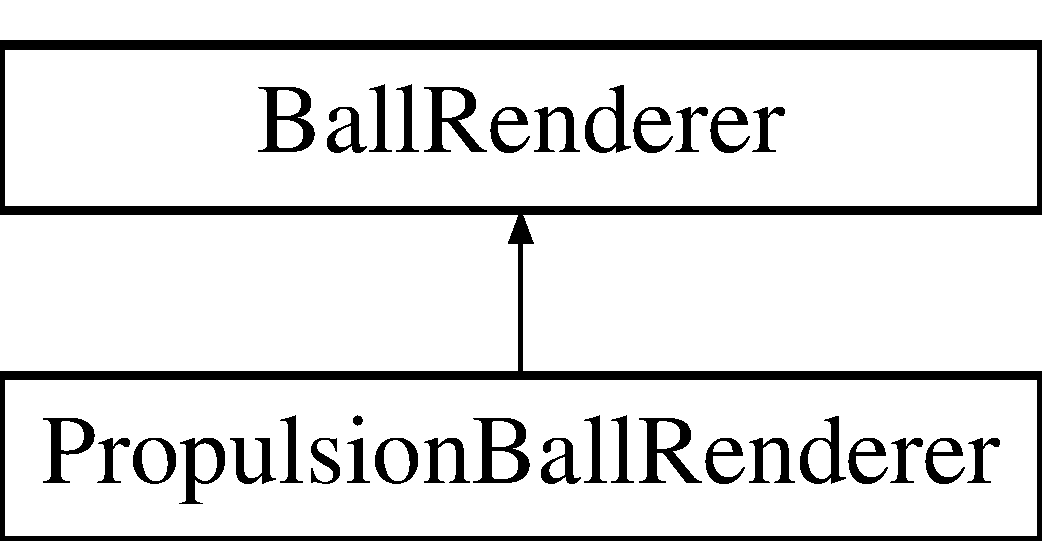
\includegraphics[height=2cm]{classPropulsionBallRenderer}
\end{center}
\end{figure}
\subsection*{Public Member Functions}
\begin{DoxyCompactItemize}
\item 
virtual void \hyperlink{classPropulsionBallRenderer_ad3206abdc61b39c3716eed6ed91acaa0}{renderBalls} (\hyperlink{classRandini_1_1SpriteLoader}{Randini::SpriteLoader} \&\_\-spriteLoader, const std::vector$<$ \hyperlink{structBall}{Ball} $>$ \&\_\-balls, const glm::mat4 \&\_\-projectionMatrix)
\begin{DoxyCompactList}\small\item\em renderBalls Since it inherits from renderballs add it to public. Unfortunately override was a c++11 so there's no way to ensure of this \item\end{DoxyCompactList}\end{DoxyCompactItemize}


\subsection{Detailed Description}
\hyperlink{classPropulsionBallRenderer}{PropulsionBallRenderer} The \hyperlink{classPropulsionBallRenderer}{PropulsionBallRenderer} class When balls increase in velocity they become brighter Set new renderer using same elements from renderBalls but altered inherits the virtual function. 

\subsection{Member Function Documentation}
\hypertarget{classPropulsionBallRenderer_ad3206abdc61b39c3716eed6ed91acaa0}{
\index{PropulsionBallRenderer@{PropulsionBallRenderer}!renderBalls@{renderBalls}}
\index{renderBalls@{renderBalls}!PropulsionBallRenderer@{PropulsionBallRenderer}}
\subsubsection[{renderBalls}]{\setlength{\rightskip}{0pt plus 5cm}void PropulsionBallRenderer::renderBalls ({\bf Randini::SpriteLoader} \& {\em \_\-spriteLoader}, \/  const std::vector$<$ {\bf Ball} $>$ \& {\em \_\-balls}, \/  const glm::mat4 \& {\em \_\-projectionMatrix})\hspace{0.3cm}{\ttfamily  \mbox{[}virtual\mbox{]}}}}
\label{classPropulsionBallRenderer_ad3206abdc61b39c3716eed6ed91acaa0}


renderBalls Since it inherits from renderballs add it to public. Unfortunately override was a c++11 so there's no way to ensure of this 
\begin{DoxyParams}{Parameters}
\item[{\em \_\-spriteLoader}]Imports the spriteLoader so it canrender balls with new renderer \item[{\em \_\-balls}]Takes the data of balls to allow them to be rendered \item[{\em \_\-projectionMatrix}]Grabs camera matrix as its needed for the uniform sampler \end{DoxyParams}


FOLLOWS SAME BASIC PRINCIPLE FROM RENDERBALLS 

Reimplemented from \hyperlink{classBallRenderer_a11d6402983ed53ab7f3d3353244110da}{BallRenderer}.

The documentation for this class was generated from the following files:\begin{DoxyCompactItemize}
\item 
Include/BallGame/\hyperlink{BallRenderer_8h}{BallRenderer.h}\item 
src/Uni/\hyperlink{BallRenderer_8cpp}{BallRenderer.cpp}\end{DoxyCompactItemize}

\hypertarget{classRandini_1_1RenderLoader}{
\section{Randini::RenderLoader Class Reference}
\label{classRandini_1_1RenderLoader}\index{Randini::RenderLoader@{Randini::RenderLoader}}
}
\subsection*{Public Member Functions}
\begin{DoxyCompactItemize}
\item 
\hypertarget{classRandini_1_1RenderLoader_ab6e4698f79e43ddc17780a5d6f69c3c8}{
{\bfseries RenderLoader} (GLuint Offset, GLuint NumVertices, GLuint Texture)}
\label{classRandini_1_1RenderLoader_ab6e4698f79e43ddc17780a5d6f69c3c8}

\end{DoxyCompactItemize}
\subsection*{Public Attributes}
\begin{DoxyCompactItemize}
\item 
\hypertarget{classRandini_1_1RenderLoader_a5eb73d19737ad1333fdec18f66f7a111}{
GLuint {\bfseries offset}}
\label{classRandini_1_1RenderLoader_a5eb73d19737ad1333fdec18f66f7a111}

\item 
\hypertarget{classRandini_1_1RenderLoader_a30bd4b7e30020ccb8c1684c25cb51451}{
GLuint {\bfseries numVertices}}
\label{classRandini_1_1RenderLoader_a30bd4b7e30020ccb8c1684c25cb51451}

\item 
\hypertarget{classRandini_1_1RenderLoader_aa7f1e320201f3b9b7e0c90799ca4b362}{
GLuint {\bfseries texture}}
\label{classRandini_1_1RenderLoader_aa7f1e320201f3b9b7e0c90799ca4b362}

\end{DoxyCompactItemize}


The documentation for this class was generated from the following file:\begin{DoxyCompactItemize}
\item 
Include/Randini/\hyperlink{SpriteLoader_8h}{SpriteLoader.h}\end{DoxyCompactItemize}

\hypertarget{classRandini_1_1ResourceManager}{
\section{Randini::ResourceManager Class Reference}
\label{classRandini_1_1ResourceManager}\index{Randini::ResourceManager@{Randini::ResourceManager}}
}
\subsection*{Static Public Member Functions}
\begin{DoxyCompactItemize}
\item 
static \hyperlink{structRandini_1_1GLTexture}{GLTexture} \hyperlink{classRandini_1_1ResourceManager_a9d7e62e883e8cdd3a7c73f5ebe9a271f}{getTexture} (std::string texturePath)
\begin{DoxyCompactList}\small\item\em getTexture follows the same priciples as the texture chace and calls it \item\end{DoxyCompactList}\end{DoxyCompactItemize}


\subsection{Member Function Documentation}
\hypertarget{classRandini_1_1ResourceManager_a9d7e62e883e8cdd3a7c73f5ebe9a271f}{
\index{Randini::ResourceManager@{Randini::ResourceManager}!getTexture@{getTexture}}
\index{getTexture@{getTexture}!Randini::ResourceManager@{Randini::ResourceManager}}
\subsubsection[{getTexture}]{\setlength{\rightskip}{0pt plus 5cm}{\bf GLTexture} Randini::ResourceManager::getTexture (std::string {\em texturePath})\hspace{0.3cm}{\ttfamily  \mbox{[}static\mbox{]}}}}
\label{classRandini_1_1ResourceManager_a9d7e62e883e8cdd3a7c73f5ebe9a271f}


getTexture follows the same priciples as the texture chace and calls it 
\begin{DoxyParams}{Parameters}
\item[{\em texturePath}]Gets the texture path from the texturecache \end{DoxyParams}
\begin{DoxyReturn}{Returns}
Texturepath of the texture from the texturecache 
\end{DoxyReturn}


The documentation for this class was generated from the following files:\begin{DoxyCompactItemize}
\item 
Include/Randini/\hyperlink{ResourceManager_8h}{ResourceManager.h}\item 
src/Randini/\hyperlink{ResourceManager_8cpp}{ResourceManager.cpp}\end{DoxyCompactItemize}

\hypertarget{classRandini_1_1SpriteLoader}{
\section{Randini::SpriteLoader Class Reference}
\label{classRandini_1_1SpriteLoader}\index{Randini::SpriteLoader@{Randini::SpriteLoader}}
}
\subsection*{Public Member Functions}
\begin{DoxyCompactItemize}
\item 
\hypertarget{classRandini_1_1SpriteLoader_a1929e27cf379b3b957b1acc5362b7331}{
void \hyperlink{classRandini_1_1SpriteLoader_a1929e27cf379b3b957b1acc5362b7331}{init} ()}
\label{classRandini_1_1SpriteLoader_a1929e27cf379b3b957b1acc5362b7331}

\begin{DoxyCompactList}\small\item\em init Inits the sprite loader and creats vertex array \item\end{DoxyCompactList}\item 
void \hyperlink{classRandini_1_1SpriteLoader_af4e355ad05c95b85af373d4f3d5a9c30}{begin} (GlyphSortType sortType=GlyphSortType::TEXTURE)
\begin{DoxyCompactList}\small\item\em calls for whenever we are ready to call sets up everything for drawing \item\end{DoxyCompactList}\item 
\hypertarget{classRandini_1_1SpriteLoader_af13de8f51b5c6428751cf417aa8efdc8}{
void \hyperlink{classRandini_1_1SpriteLoader_af13de8f51b5c6428751cf417aa8efdc8}{end} ()}
\label{classRandini_1_1SpriteLoader_af13de8f51b5c6428751cf417aa8efdc8}

\begin{DoxyCompactList}\small\item\em end used to sort the glyyphs and genrate batched for the glyphs \item\end{DoxyCompactList}\item 
void \hyperlink{classRandini_1_1SpriteLoader_acfb6c713ca114db19e1b724ed08fc645}{draw} (const glm::vec4 \&destinationRect, glm::vec4 \&uvRect, GLuint texture, float depth, const \hyperlink{structRandini_1_1ColorRGBA8}{ColorRGBA8} \&color)
\begin{DoxyCompactList}\small\item\em draw calls void draw through void begin and adds the sprites to the batch and gets them ready to load use glm over SDL Rect so I can import the math easier makes them a const so the reference does not change. prevent copys and increase speed. Make them destination const to prevent values changing \item\end{DoxyCompactList}\item 
\hypertarget{classRandini_1_1SpriteLoader_ad552f49e04affcffc57936ff1b6c2cc0}{
void \hyperlink{classRandini_1_1SpriteLoader_ad552f49e04affcffc57936ff1b6c2cc0}{renderLoader} ()}
\label{classRandini_1_1SpriteLoader_ad552f49e04affcffc57936ff1b6c2cc0}

\begin{DoxyCompactList}\small\item\em renderLoader renders the sprites to the screen and binds them together for rendering \item\end{DoxyCompactList}\end{DoxyCompactItemize}


\subsection{Member Function Documentation}
\hypertarget{classRandini_1_1SpriteLoader_af4e355ad05c95b85af373d4f3d5a9c30}{
\index{Randini::SpriteLoader@{Randini::SpriteLoader}!begin@{begin}}
\index{begin@{begin}!Randini::SpriteLoader@{Randini::SpriteLoader}}
\subsubsection[{begin}]{\setlength{\rightskip}{0pt plus 5cm}void Randini::SpriteLoader::begin (GlyphSortType {\em sortType} = {\ttfamily GlyphSortType::TEXTURE})}}
\label{classRandini_1_1SpriteLoader_af4e355ad05c95b85af373d4f3d5a9c30}


calls for whenever we are ready to call sets up everything for drawing 
\begin{DoxyParams}{Parameters}
\item[{\em sortType}]Sets up sorting process for whenever begin is called to begin rendering \end{DoxyParams}
\hypertarget{classRandini_1_1SpriteLoader_acfb6c713ca114db19e1b724ed08fc645}{
\index{Randini::SpriteLoader@{Randini::SpriteLoader}!draw@{draw}}
\index{draw@{draw}!Randini::SpriteLoader@{Randini::SpriteLoader}}
\subsubsection[{draw}]{\setlength{\rightskip}{0pt plus 5cm}void Randini::SpriteLoader::draw (const glm::vec4 \& {\em destinationRect}, \/  glm::vec4 \& {\em uvRect}, \/  GLuint {\em texture}, \/  float {\em depth}, \/  const {\bf ColorRGBA8} \& {\em color})}}
\label{classRandini_1_1SpriteLoader_acfb6c713ca114db19e1b724ed08fc645}


draw calls void draw through void begin and adds the sprites to the batch and gets them ready to load use glm over SDL Rect so I can import the math easier makes them a const so the reference does not change. prevent copys and increase speed. Make them destination const to prevent values changing 
\begin{DoxyParams}{Parameters}
\item[{\em destinationRect}]position stored at of the sprite \item[{\em uvRect}]uv coordinates with bottom left hand cornor and dimensions \item[{\em texture}]texture storage \item[{\em depth}]depth of the texture \item[{\em color}]Color of the sprite \end{DoxyParams}


The documentation for this class was generated from the following files:\begin{DoxyCompactItemize}
\item 
Include/Randini/\hyperlink{SpriteLoader_8h}{SpriteLoader.h}\item 
src/Randini/SpriteLoader.cpp\end{DoxyCompactItemize}

\hypertarget{classRandini_1_1TextureCache}{
\section{Randini::TextureCache Class Reference}
\label{classRandini_1_1TextureCache}\index{Randini::TextureCache@{Randini::TextureCache}}
}
\subsection*{Public Member Functions}
\begin{DoxyCompactItemize}
\item 
\hyperlink{structRandini_1_1GLTexture}{GLTexture} \hyperlink{classRandini_1_1TextureCache_a616aab3abb7b12c93ab9204432e9512d}{getTexture} (std::string texturePath)
\begin{DoxyCompactList}\small\item\em getTexture returns \hyperlink{structRandini_1_1GLTexture}{GLTexture}. Look up in the map and see if the texture is there if it is then it will just return the existing texture the texture internally stores the GLuint ID which is a pointer to the actual texture if it dosent create a new which will push it back onto the texture map. \item\end{DoxyCompactList}\end{DoxyCompactItemize}


\subsection{Member Function Documentation}
\hypertarget{classRandini_1_1TextureCache_a616aab3abb7b12c93ab9204432e9512d}{
\index{Randini::TextureCache@{Randini::TextureCache}!getTexture@{getTexture}}
\index{getTexture@{getTexture}!Randini::TextureCache@{Randini::TextureCache}}
\subsubsection[{getTexture}]{\setlength{\rightskip}{0pt plus 5cm}{\bf GLTexture} Randini::TextureCache::getTexture (std::string {\em texturePath})}}
\label{classRandini_1_1TextureCache_a616aab3abb7b12c93ab9204432e9512d}


getTexture returns \hyperlink{structRandini_1_1GLTexture}{GLTexture}. Look up in the map and see if the texture is there if it is then it will just return the existing texture the texture internally stores the GLuint ID which is a pointer to the actual texture if it dosent create a new which will push it back onto the texture map. 
\begin{DoxyParams}{Parameters}
\item[{\em texturePath}]Gets the texturepath from the texturemap and adds it if its not there\end{DoxyParams}
\begin{DoxyReturn}{Returns}
//since mit is not pointing to texturemap.end it is pointing to the texture //Therefore return mit to the second pair which will return the texture 
\end{DoxyReturn}


The documentation for this class was generated from the following files:\begin{DoxyCompactItemize}
\item 
Include/Randini/\hyperlink{TextureCache_8h}{TextureCache.h}\item 
src/Randini/\hyperlink{TextureCache_8cpp}{TextureCache.cpp}\end{DoxyCompactItemize}

\hypertarget{structRandini_1_1UV}{
\section{Randini::UV Struct Reference}
\label{structRandini_1_1UV}\index{Randini::UV@{Randini::UV}}
}
\subsection*{Public Attributes}
\begin{DoxyCompactItemize}
\item 
\hypertarget{structRandini_1_1UV_a91db8093ca6754e5dd3e536de44d4cc3}{
float {\bfseries u}}
\label{structRandini_1_1UV_a91db8093ca6754e5dd3e536de44d4cc3}

\item 
\hypertarget{structRandini_1_1UV_a02bd106502066df36e4115c7408e8afd}{
float {\bfseries v}}
\label{structRandini_1_1UV_a02bd106502066df36e4115c7408e8afd}

\end{DoxyCompactItemize}


The documentation for this struct was generated from the following file:\begin{DoxyCompactItemize}
\item 
Include/Randini/\hyperlink{Vertex_8h}{Vertex.h}\end{DoxyCompactItemize}

\hypertarget{classVelocityBallRendererX}{
\section{VelocityBallRendererX Class Reference}
\label{classVelocityBallRendererX}\index{VelocityBallRendererX@{VelocityBallRendererX}}
}


{\ttfamily \#include $<$BallRenderer.h$>$}Inheritance diagram for VelocityBallRendererX::\begin{figure}[H]
\begin{center}
\leavevmode
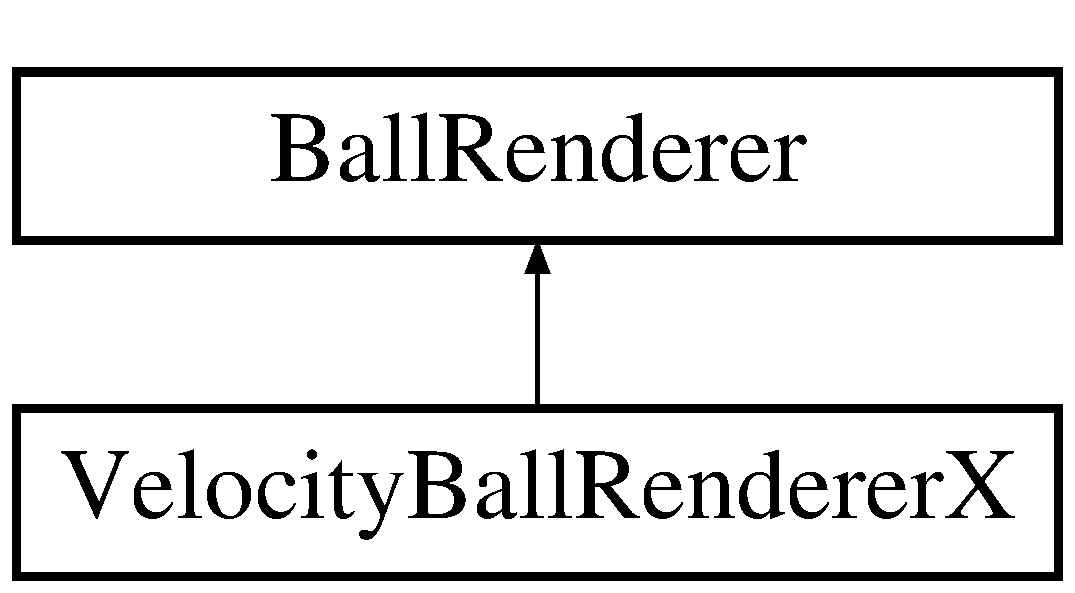
\includegraphics[height=2cm]{classVelocityBallRendererX}
\end{center}
\end{figure}
\subsection*{Public Member Functions}
\begin{DoxyCompactItemize}
\item 
\hypertarget{classVelocityBallRendererX_ad3ae42e2ab2efab70a9812267eb337a7}{
{\bfseries VelocityBallRendererX} (int screenWidth, int screenHeight)}
\label{classVelocityBallRendererX_ad3ae42e2ab2efab70a9812267eb337a7}

\item 
virtual void \hyperlink{classVelocityBallRendererX_ad0ef24ce7ba5116231f4a47aff280f12}{renderBalls} (\hyperlink{classRandini_1_1SpriteLoader}{Randini::SpriteLoader} \&spriteLoader, const std::vector$<$ \hyperlink{structBall}{Ball} $>$ \&balls, const glm::mat4 \&projectionMatrix)
\end{DoxyCompactItemize}


\subsection{Detailed Description}
Visualise the velocity of ball renderers when moving in the x direction as well as visualise the position with different colours 

\subsection{Member Function Documentation}
\hypertarget{classVelocityBallRendererX_ad0ef24ce7ba5116231f4a47aff280f12}{
\index{VelocityBallRendererX@{VelocityBallRendererX}!renderBalls@{renderBalls}}
\index{renderBalls@{renderBalls}!VelocityBallRendererX@{VelocityBallRendererX}}
\subsubsection[{renderBalls}]{\setlength{\rightskip}{0pt plus 5cm}void VelocityBallRendererX::renderBalls ({\bf Randini::SpriteLoader} \& {\em spriteLoader}, \/  const std::vector$<$ {\bf Ball} $>$ \& {\em balls}, \/  const glm::mat4 \& {\em projectionMatrix})\hspace{0.3cm}{\ttfamily  \mbox{[}virtual\mbox{]}}}}
\label{classVelocityBallRendererX_ad0ef24ce7ba5116231f4a47aff280f12}
Make this a virtual function as I want to derive form this Imports the sprites from the game engine renders a list of balls to render all the balls Instead of rendering a single ball loop through all the balls 

FOLLOWS SAME BASIC PRINCIPLE FROM RENDERBALLS 

Reimplemented from \hyperlink{classBallRenderer_a6169ba2a00e8d15fde87a3ee4552cf66}{BallRenderer}.

The documentation for this class was generated from the following files:\begin{DoxyCompactItemize}
\item 
Include/BallGame/\hyperlink{BallRenderer_8h}{BallRenderer.h}\item 
src/Uni/\hyperlink{BallRenderer_8cpp}{BallRenderer.cpp}\end{DoxyCompactItemize}

\hypertarget{classVelocityBallRendererY}{
\section{VelocityBallRendererY Class Reference}
\label{classVelocityBallRendererY}\index{VelocityBallRendererY@{VelocityBallRendererY}}
}


{\ttfamily \#include $<$BallRenderer.h$>$}Inheritance diagram for VelocityBallRendererY::\begin{figure}[H]
\begin{center}
\leavevmode
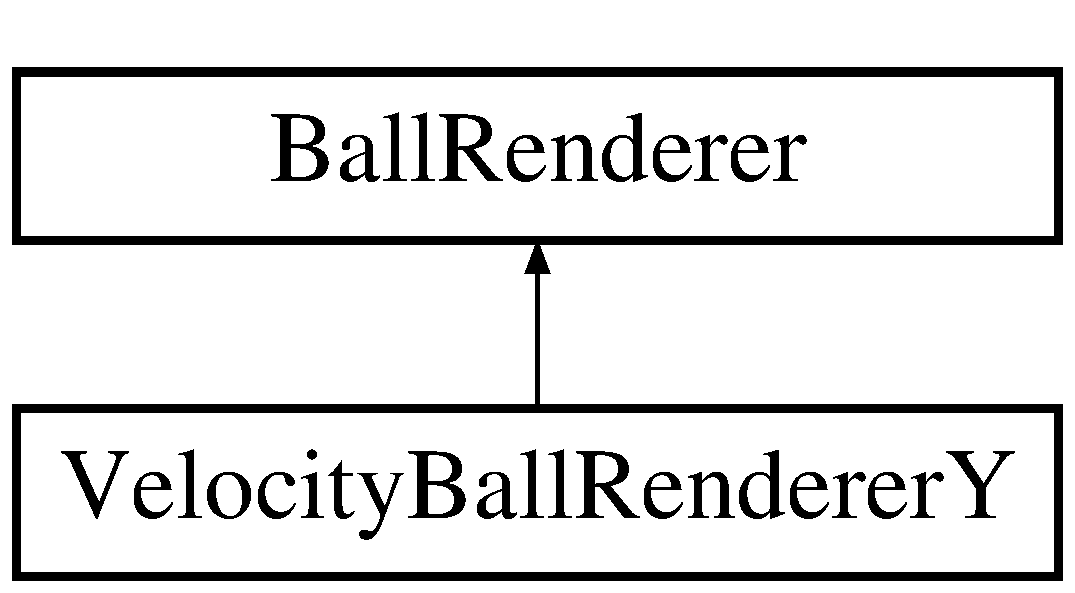
\includegraphics[height=2cm]{classVelocityBallRendererY}
\end{center}
\end{figure}
\subsection*{Public Member Functions}
\begin{DoxyCompactItemize}
\item 
\hypertarget{classVelocityBallRendererY_acbe922bfa2f2280299d9cb4a0d823395}{
{\bfseries VelocityBallRendererY} (int screenWidth, int screenHeight)}
\label{classVelocityBallRendererY_acbe922bfa2f2280299d9cb4a0d823395}

\item 
virtual void \hyperlink{classVelocityBallRendererY_aee5499c81382f071f58467d2040e36c9}{renderBalls} (\hyperlink{classRandini_1_1SpriteLoader}{Randini::SpriteLoader} \&spriteLoader, const std::vector$<$ \hyperlink{structBall}{Ball} $>$ \&balls, const glm::mat4 \&projectionMatrix)
\end{DoxyCompactItemize}


\subsection{Detailed Description}
Visualise the velocity of ball renderers when moving in the y direction as well as visualise the position with different colours 

\subsection{Member Function Documentation}
\hypertarget{classVelocityBallRendererY_aee5499c81382f071f58467d2040e36c9}{
\index{VelocityBallRendererY@{VelocityBallRendererY}!renderBalls@{renderBalls}}
\index{renderBalls@{renderBalls}!VelocityBallRendererY@{VelocityBallRendererY}}
\subsubsection[{renderBalls}]{\setlength{\rightskip}{0pt plus 5cm}void VelocityBallRendererY::renderBalls ({\bf Randini::SpriteLoader} \& {\em spriteLoader}, \/  const std::vector$<$ {\bf Ball} $>$ \& {\em balls}, \/  const glm::mat4 \& {\em projectionMatrix})\hspace{0.3cm}{\ttfamily  \mbox{[}virtual\mbox{]}}}}
\label{classVelocityBallRendererY_aee5499c81382f071f58467d2040e36c9}
Make this a virtual function as I want to derive form this Imports the sprites from the game engine renders a list of balls to render all the balls Instead of rendering a single ball loop through all the balls 

Reimplemented from \hyperlink{classBallRenderer_a6169ba2a00e8d15fde87a3ee4552cf66}{BallRenderer}.

The documentation for this class was generated from the following files:\begin{DoxyCompactItemize}
\item 
Include/BallGame/\hyperlink{BallRenderer_8h}{BallRenderer.h}\item 
src/Uni/\hyperlink{BallRenderer_8cpp}{BallRenderer.cpp}\end{DoxyCompactItemize}

\hypertarget{structRandini_1_1Vertex}{
\section{Randini::Vertex Struct Reference}
\label{structRandini_1_1Vertex}\index{Randini::Vertex@{Randini::Vertex}}
}
\subsection*{Public Member Functions}
\begin{DoxyCompactItemize}
\item 
\hypertarget{structRandini_1_1Vertex_ad00ffb3af37c668d40f28ae2d8cce41b}{
void {\bfseries setPosition} (float x, float y)}
\label{structRandini_1_1Vertex_ad00ffb3af37c668d40f28ae2d8cce41b}

\item 
\hypertarget{structRandini_1_1Vertex_a1433f80829a7d1c3486ac9ef669e3e76}{
void {\bfseries setUV} (float u, float v)}
\label{structRandini_1_1Vertex_a1433f80829a7d1c3486ac9ef669e3e76}

\end{DoxyCompactItemize}
\subsection*{Public Attributes}
\begin{DoxyCompactItemize}
\item 
\hypertarget{structRandini_1_1Vertex_ae5335415f2c18745710786492093b37c}{
\hyperlink{structRandini_1_1Position}{Position} {\bfseries position}}
\label{structRandini_1_1Vertex_ae5335415f2c18745710786492093b37c}

\item 
\hypertarget{structRandini_1_1Vertex_a47ba3de5e86302c30d50051d840cd4a9}{
\hyperlink{structRandini_1_1ColorRGBA8}{ColorRGBA8} {\bfseries color}}
\label{structRandini_1_1Vertex_a47ba3de5e86302c30d50051d840cd4a9}

\item 
\hypertarget{structRandini_1_1Vertex_a72d59c20270fb7777ae6e0457fe6d1b9}{
\hyperlink{structRandini_1_1UV}{UV} {\bfseries uv}}
\label{structRandini_1_1Vertex_a72d59c20270fb7777ae6e0457fe6d1b9}

\end{DoxyCompactItemize}


The documentation for this struct was generated from the following file:\begin{DoxyCompactItemize}
\item 
Include/Randini/\hyperlink{Vertex_8h}{Vertex.h}\end{DoxyCompactItemize}

\hypertarget{classRandini_1_1Window}{
\section{Randini::Window Class Reference}
\label{classRandini_1_1Window}\index{Randini::Window@{Randini::Window}}
}
\subsection*{Public Member Functions}
\begin{DoxyCompactItemize}
\item 
\hypertarget{classRandini_1_1Window_a74f33cf737af665902138f80cc779cb5}{
int {\bfseries create} (std::string windowName, int screenWidth, int screenHeight, unsigned int currentFlags)}
\label{classRandini_1_1Window_a74f33cf737af665902138f80cc779cb5}

\item 
\hypertarget{classRandini_1_1Window_af0fe0a4f666f5c946bb8df997977e40e}{
void {\bfseries swapBuffers} ()}
\label{classRandini_1_1Window_af0fe0a4f666f5c946bb8df997977e40e}

\item 
\hypertarget{classRandini_1_1Window_a7b4ddf85609bbe27f2800ff05a0130dc}{
int {\bfseries getScreenWidth} ()}
\label{classRandini_1_1Window_a7b4ddf85609bbe27f2800ff05a0130dc}

\item 
\hypertarget{classRandini_1_1Window_aedbf196a50a63cf91c8eedcc5d80e204}{
int {\bfseries getScreenHeight} ()}
\label{classRandini_1_1Window_aedbf196a50a63cf91c8eedcc5d80e204}

\end{DoxyCompactItemize}


The documentation for this class was generated from the following files:\begin{DoxyCompactItemize}
\item 
Include/Randini/\hyperlink{Window_8h}{Window.h}\item 
src/Randini/\hyperlink{Window_8cpp}{Window.cpp}\end{DoxyCompactItemize}

\chapter{File Documentation}
\hypertarget{Ball_8h}{
\section{Include/BallGame/Ball.h File Reference}
\label{Ball_8h}\index{Include/BallGame/Ball.h@{Include/BallGame/Ball.h}}
}


Handle the data for the ball.  
{\ttfamily \#include $<$glm/glm.hpp$>$}\par
{\ttfamily \#include $<$Include/Randini/Vertex.h$>$}\par
\subsection*{Classes}
\begin{DoxyCompactItemize}
\item 
struct \hyperlink{structBall}{Ball}
\end{DoxyCompactItemize}


\subsection{Detailed Description}
Handle the data for the ball. \begin{DoxyVersion}{Version}
1.0 
\end{DoxyVersion}
\begin{DoxyAuthor}{Author}
Philip Gifford 
\end{DoxyAuthor}
\begin{DoxyDate}{Date}
02/05/15 
\end{DoxyDate}

\hypertarget{BallControl_8h}{
\section{Include/BallGame/BallControl.h File Reference}
\label{BallControl_8h}\index{Include/BallGame/BallControl.h@{Include/BallGame/BallControl.h}}
}


Handle different ball controls and tracks mouse for grabbing.  
{\ttfamily \#include $<$vector$>$}\par
{\ttfamily \#include \char`\"{}Ball.h\char`\"{}}\par
\subsection*{Classes}
\begin{DoxyCompactItemize}
\item 
class \hyperlink{classBallControl}{BallControl}
\item 
class \hyperlink{classColorTransferControl}{ColorTransferControl}
\end{DoxyCompactItemize}
\subsection*{Enumerations}
\begin{DoxyCompactItemize}
\item 
enum {\bfseries GravityControl} \{ \par
{\bfseries NONE}, 
{\bfseries LEFT}, 
{\bfseries UP}, 
{\bfseries RIGHT}, 
\par
{\bfseries DOWN}
 \}
\end{DoxyCompactItemize}


\subsection{Detailed Description}
Handle different ball controls and tracks mouse for grabbing. \begin{DoxyVersion}{Version}
1.0 
\end{DoxyVersion}
\begin{DoxyAuthor}{Author}
Philip Gifford 
\end{DoxyAuthor}
\begin{DoxyDate}{Date}
02/05/15 
\end{DoxyDate}

\hypertarget{BallGrid_8h}{
\section{Include/BallGame/BallGrid.h File Reference}
\label{BallGrid_8h}\index{Include/BallGame/BallGrid.h@{Include/BallGame/BallGrid.h}}
}


Imports the grid/cells to store balls in for spatial partioning.  
{\ttfamily \#include \char`\"{}Ball.h\char`\"{}}\par
{\ttfamily \#include $<$vector$>$}\par
\subsection*{Classes}
\begin{DoxyCompactItemize}
\item 
struct \hyperlink{structCell}{Cell}
\begin{DoxyCompactList}\small\item\em Inlcude vector as using vector for the list. \item\end{DoxyCompactList}\item 
class \hyperlink{classBallGrid}{BallGrid}
\end{DoxyCompactItemize}


\subsection{Detailed Description}
Imports the grid/cells to store balls in for spatial partioning. \begin{DoxyVersion}{Version}
1.0 
\end{DoxyVersion}
\begin{DoxyAuthor}{Author}
Philip Gifford 
\end{DoxyAuthor}
\begin{DoxyDate}{Date}
02/05/15 
\end{DoxyDate}

\hypertarget{BallRenderer_8h}{
\section{Include/BallGame/BallRenderer.h File Reference}
\label{BallRenderer_8h}\index{Include/BallGame/BallRenderer.h@{Include/BallGame/BallRenderer.h}}
}


Contolrs different renders and inits the shaders and textures.  
{\ttfamily \#include $<$Include/Randini/SpriteLoader.h$>$}\par
{\ttfamily \#include $<$Include/Randini/GLSLProgram.h$>$}\par
{\ttfamily \#include $<$memory$>$}\par
{\ttfamily \#include $<$vector$>$}\par
{\ttfamily \#include \char`\"{}Ball.h\char`\"{}}\par
\subsection*{Classes}
\begin{DoxyCompactItemize}
\item 
class \hyperlink{classBallRenderer}{BallRenderer}
\item 
class \hyperlink{classPropulsionBallRenderer}{PropulsionBallRenderer}
\item 
class \hyperlink{classVelocityBallRendererX}{VelocityBallRendererX}
\item 
class \hyperlink{classVelocityBallRendererY}{VelocityBallRendererY}
\end{DoxyCompactItemize}


\subsection{Detailed Description}
Contolrs different renders and inits the shaders and textures. \begin{DoxyVersion}{Version}
1.0 
\end{DoxyVersion}
\begin{DoxyAuthor}{Author}
Philip Gifford 
\end{DoxyAuthor}
\begin{DoxyDate}{Date}
02/05/15 
\end{DoxyDate}

\hypertarget{MainGame_8h}{
\section{Include/BallGame/MainGame.h File Reference}
\label{MainGame_8h}\index{Include/BallGame/MainGame.h@{Include/BallGame/MainGame.h}}
}


Calls functions from Randini Engine \& deals with key input, drawing, deltatime.  
{\ttfamily \#include $<$Include/Randini/Camera2D.h$>$}\par
{\ttfamily \#include $<$Include/Randini/SpriteLoader.h$>$}\par
{\ttfamily \#include $<$Include/Randini/InputControl.h$>$}\par
{\ttfamily \#include $<$Include/Randini/Window.h$>$}\par
{\ttfamily \#include $<$Include/Randini/GLSLProgram.h$>$}\par
{\ttfamily \#include $<$Include/Randini/Timer.h$>$}\par
{\ttfamily \#include $<$memory$>$}\par
{\ttfamily \#include $<$utility$>$}\par
{\ttfamily \#include \char`\"{}BallControl.h\char`\"{}}\par
{\ttfamily \#include \char`\"{}BallRenderer.h\char`\"{}}\par
{\ttfamily \#include \char`\"{}BallGrid.h\char`\"{}}\par
{\ttfamily \#include \char`\"{}boost/random.hpp\char`\"{}}\par
{\ttfamily \#include \char`\"{}boost/generator\_\-iterator.hpp\char`\"{}}\par
\subsection*{Classes}
\begin{DoxyCompactItemize}
\item 
class \hyperlink{classMainGame}{MainGame}
\end{DoxyCompactItemize}
\subsection*{Typedefs}
\begin{DoxyCompactItemize}
\item 
typedef boost::uniform\_\-real$<$ float $>$ \hyperlink{MainGame_8h_a3bbd6868c609bd755d6336c79fad44aa}{RandomDistribution}
\item 
\hypertarget{MainGame_8h_a643e304c4c67358cc9dc9414165dea85}{
typedef boost::uniform\_\-int$<$ int $>$ {\bfseries RandomDistributionInt}}
\label{MainGame_8h_a643e304c4c67358cc9dc9414165dea85}

\item 
\hypertarget{MainGame_8h_a0f7898448a7748cac3877d1f5c445dac}{
typedef boost::mt19937 {\bfseries RNGType}}
\label{MainGame_8h_a0f7898448a7748cac3877d1f5c445dac}

\end{DoxyCompactItemize}
\subsection*{Enumerations}
\begin{DoxyCompactItemize}
\item 
enum \hyperlink{MainGame_8h_a7899b65f1ea0f655e4bbf8d2a5714285}{GameState} \{ {\bfseries PLAY}, 
{\bfseries EXIT}
 \}
\begin{DoxyCompactList}\small\item\em basic enum for gamestate \item\end{DoxyCompactList}\end{DoxyCompactItemize}
\subsection*{Variables}
\begin{DoxyCompactItemize}
\item 
\hypertarget{MainGame_8h_a3d75a3045c57e393b76a1760deb2533c}{
const int {\bfseries CELL\_\-SIZE} = 12}
\label{MainGame_8h_a3d75a3045c57e393b76a1760deb2533c}

\end{DoxyCompactItemize}


\subsection{Detailed Description}
Calls functions from Randini Engine \& deals with key input, drawing, deltatime. \begin{DoxyVersion}{Version}
1.0 
\end{DoxyVersion}
\begin{DoxyAuthor}{Author}
Philip Gifford 
\end{DoxyAuthor}
\begin{DoxyDate}{Date}
02/05/15 
\end{DoxyDate}


\subsection{Typedef Documentation}
\hypertarget{MainGame_8h_a3bbd6868c609bd755d6336c79fad44aa}{
\index{MainGame.h@{MainGame.h}!RandomDistribution@{RandomDistribution}}
\index{RandomDistribution@{RandomDistribution}!MainGame.h@{MainGame.h}}
\subsubsection[{RandomDistribution}]{\setlength{\rightskip}{0pt plus 5cm}typedef boost::uniform\_\-real$<$float$>$ {\bf RandomDistribution}}}
\label{MainGame_8h_a3bbd6868c609bd755d6336c79fad44aa}
add boost to add imporved random libary. set each different call to certain name 
\hypertarget{Camera2D_8h}{
\section{Include/Randini/Camera2D.h File Reference}
\label{Camera2D_8h}\index{Include/Randini/Camera2D.h@{Include/Randini/Camera2D.h}}
}


Creates the camera gains screen coordinates and returns the camera position.  
{\ttfamily \#include $<$glm/glm.hpp$>$}\par
{\ttfamily \#include $<$glm/gtc/matrix\_\-transform.hpp$>$}\par
\subsection*{Classes}
\begin{DoxyCompactItemize}
\item 
class \hyperlink{classRandini_1_1Camera2D}{Randini::Camera2D}
\end{DoxyCompactItemize}


\subsection{Detailed Description}
Creates the camera gains screen coordinates and returns the camera position. \begin{DoxyVersion}{Version}
1.0 
\end{DoxyVersion}
\begin{DoxyAuthor}{Author}
Philip Gifford 
\end{DoxyAuthor}
\begin{DoxyDate}{Date}
02/05/15 
\end{DoxyDate}

\hypertarget{GLSLProgram_8h}{
\section{Include/Randini/GLSLProgram.h File Reference}
\label{GLSLProgram_8h}\index{Include/Randini/GLSLProgram.h@{Include/Randini/GLSLProgram.h}}
}


Compiles, Links, Enables, \& Disables frag and vert shaders and returns the location of the uniform.  
{\ttfamily \#include $<$iostream$>$}\par
{\ttfamily \#include $<$string$>$}\par
{\ttfamily \#include $<$GL/glew.h$>$}\par
\subsection*{Classes}
\begin{DoxyCompactItemize}
\item 
class \hyperlink{classRandini_1_1GLSLProgram}{Randini::GLSLProgram}
\end{DoxyCompactItemize}


\subsection{Detailed Description}
Compiles, Links, Enables, \& Disables frag and vert shaders and returns the location of the uniform. \begin{DoxyVersion}{Version}
1.0 
\end{DoxyVersion}
\begin{DoxyAuthor}{Author}
Philip Gifford 
\end{DoxyAuthor}
\begin{DoxyDate}{Date}
02/05/15 
\end{DoxyDate}

\hypertarget{GLTexture_8h}{
\section{Include/Randini/GLTexture.h File Reference}
\label{GLTexture_8h}\index{Include/Randini/GLTexture.h@{Include/Randini/GLTexture.h}}
}


Creats a struct to handle data id of textures.  
{\ttfamily \#include $<$GL/glew.h$>$}\par
\subsection*{Classes}
\begin{DoxyCompactItemize}
\item 
struct \hyperlink{structRandini_1_1GLTexture}{Randini::GLTexture}
\end{DoxyCompactItemize}


\subsection{Detailed Description}
Creats a struct to handle data id of textures. \begin{DoxyVersion}{Version}
1.0 
\end{DoxyVersion}
\begin{DoxyAuthor}{Author}
Philip Gifford 
\end{DoxyAuthor}
\begin{DoxyDate}{Date}
02/05/15 
\end{DoxyDate}

\hypertarget{ImageLoader_8h}{
\section{Include/Randini/ImageLoader.h File Reference}
\label{ImageLoader_8h}\index{Include/Randini/ImageLoader.h@{Include/Randini/ImageLoader.h}}
}


Reads a texture file and returns a GLTexture.  
{\ttfamily \#include \char`\"{}GLTexture.h\char`\"{}}\par
{\ttfamily \#include $<$string$>$}\par
\subsection*{Classes}
\begin{DoxyCompactItemize}
\item 
class \hyperlink{classRandini_1_1ImageLoader}{Randini::ImageLoader}
\end{DoxyCompactItemize}


\subsection{Detailed Description}
Reads a texture file and returns a GLTexture. \begin{DoxyVersion}{Version}
1.0 
\end{DoxyVersion}
\begin{DoxyAuthor}{Author}
Philip Gifford 
\end{DoxyAuthor}
\begin{DoxyDate}{Date}
02/05/15 
\end{DoxyDate}

\hypertarget{IOManager_8h}{
\section{Include/Randini/IOManager.h File Reference}
\label{IOManager_8h}\index{Include/Randini/IOManager.h@{Include/Randini/IOManager.h}}
}


Seeks the size of the buffer and reads the file to it returns open file.  
{\ttfamily \#include $<$vector$>$}\par
{\ttfamily \#include $<$string$>$}\par
\subsection*{Classes}
\begin{DoxyCompactItemize}
\item 
class \hyperlink{classRandini_1_1IOManager}{Randini::IOManager}
\end{DoxyCompactItemize}


\subsection{Detailed Description}
Seeks the size of the buffer and reads the file to it returns open file. \begin{DoxyVersion}{Version}
1.0 
\end{DoxyVersion}
\begin{DoxyAuthor}{Author}
Philip Gifford 
\end{DoxyAuthor}
\begin{DoxyDate}{Date}
02/05/15 
\end{DoxyDate}

\hypertarget{Randini_8h}{
\section{Include/Randini/Randini.h File Reference}
\label{Randini_8h}\index{Include/Randini/Randini.h@{Include/Randini/Randini.h}}
}


Encapsulates all data in namespace, inits everything and sets double buffer.  
\subsection*{Functions}
\begin{DoxyCompactItemize}
\item 
\hypertarget{namespaceRandini_a56b7fe6fca95ec39b0dc6cb3d6a778d6}{
int {\bfseries Randini::init} ()}
\label{namespaceRandini_a56b7fe6fca95ec39b0dc6cb3d6a778d6}

\end{DoxyCompactItemize}


\subsection{Detailed Description}
Encapsulates all data in namespace, inits everything and sets double buffer. \begin{DoxyVersion}{Version}
1.0 
\end{DoxyVersion}
\begin{DoxyAuthor}{Author}
Philip Gifford 
\end{DoxyAuthor}
\begin{DoxyDate}{Date}
02/05/15 
\end{DoxyDate}

\hypertarget{ResourceManager_8h}{
\section{Include/Randini/ResourceManager.h File Reference}
\label{ResourceManager_8h}\index{Include/Randini/ResourceManager.h@{Include/Randini/ResourceManager.h}}
}


Calls texturecache to retrieve texture path.  
{\ttfamily \#include \char`\"{}TextureCache.h\char`\"{}}\par
{\ttfamily \#include $<$string$>$}\par
\subsection*{Classes}
\begin{DoxyCompactItemize}
\item 
class \hyperlink{classRandini_1_1ResourceManager}{Randini::ResourceManager}
\end{DoxyCompactItemize}


\subsection{Detailed Description}
Calls texturecache to retrieve texture path. \begin{DoxyVersion}{Version}
1.0 
\end{DoxyVersion}
\begin{DoxyAuthor}{Author}
Philip Gifford 
\end{DoxyAuthor}
\begin{DoxyDate}{Date}
02/05/15 
\end{DoxyDate}

\hypertarget{SpriteLoader_8h}{
\section{Include/Randini/SpriteLoader.h File Reference}
\label{SpriteLoader_8h}\index{Include/Randini/SpriteLoader.h@{Include/Randini/SpriteLoader.h}}
}


Allows for multiple sprites to be drawn \& rendered. Sets vertices for glyphs.  
{\ttfamily \#include $<$GL/glew.h$>$}\par
{\ttfamily \#include \char`\"{}Vertex.h\char`\"{}}\par
{\ttfamily \#include $<$glm/glm.hpp$>$}\par
{\ttfamily \#include $<$vector$>$}\par
{\ttfamily \#include $<$utility$>$}\par
\subsection*{Classes}
\begin{DoxyCompactItemize}
\item 
class \hyperlink{classRandini_1_1Glyph}{Randini::Glyph}
\item 
class \hyperlink{classRandini_1_1RenderLoader}{Randini::RenderLoader}
\item 
class \hyperlink{classRandini_1_1SpriteLoader}{Randini::SpriteLoader}
\end{DoxyCompactItemize}
\subsection*{Enumerations}
\begin{DoxyCompactItemize}
\item 
enum {\bfseries GlyphSortType} \{ {\bfseries NONE}, 
{\bfseries FRONT\_\-TO\_\-BACK}, 
{\bfseries BACK\_\-TO\_\-FRONT}, 
{\bfseries TEXTURE}
 \}
\end{DoxyCompactItemize}


\subsection{Detailed Description}
Allows for multiple sprites to be drawn \& rendered. Sets vertices for glyphs. \begin{DoxyVersion}{Version}
1.0 
\end{DoxyVersion}
\begin{DoxyAuthor}{Author}
Philip Gifford 
\end{DoxyAuthor}
\begin{DoxyDate}{Date}
02/05/15 
\end{DoxyDate}

\hypertarget{TextureCache_8h}{
\section{Include/Randini/TextureCache.h File Reference}
\label{TextureCache_8h}\index{Include/Randini/TextureCache.h@{Include/Randini/TextureCache.h}}
}


Checks if texture is in texture map, loads new textures and creates new path. Returns new texture.  
{\ttfamily \#include $<$map$>$}\par
{\ttfamily \#include $<$string$>$}\par
{\ttfamily \#include \char`\"{}GLTexture.h\char`\"{}}\par
\subsection*{Classes}
\begin{DoxyCompactItemize}
\item 
class \hyperlink{classRandini_1_1TextureCache}{Randini::TextureCache}
\end{DoxyCompactItemize}


\subsection{Detailed Description}
Checks if texture is in texture map, loads new textures and creates new path. Returns new texture. \begin{DoxyVersion}{Version}
1.0 
\end{DoxyVersion}
\begin{DoxyAuthor}{Author}
Philip Gifford 
\end{DoxyAuthor}
\begin{DoxyDate}{Date}
02/05/15 
\end{DoxyDate}

\hypertarget{Timer_8h}{
\section{Include/Randini/Timer.h File Reference}
\label{Timer_8h}\index{Include/Randini/Timer.h@{Include/Randini/Timer.h}}
}


Calculates, monitors, and caps the FPS this allows for setting deltaTime later.  
\subsection*{Classes}
\begin{DoxyCompactItemize}
\item 
class \hyperlink{classRandini_1_1FPSLimiter}{Randini::FPSLimiter}
\end{DoxyCompactItemize}


\subsection{Detailed Description}
Calculates, monitors, and caps the FPS this allows for setting deltaTime later. \begin{DoxyVersion}{Version}
1.0 
\end{DoxyVersion}
\begin{DoxyAuthor}{Author}
Philip Gifford 
\end{DoxyAuthor}
\begin{DoxyDate}{Date}
02/05/15 
\end{DoxyDate}

\hypertarget{Vertex_8h}{
\section{Include/Randini/Vertex.h File Reference}
\label{Vertex_8h}\index{Include/Randini/Vertex.h@{Include/Randini/Vertex.h}}
}


Handle the data for the ball.  
{\ttfamily \#include $<$GL/glew.h$>$}\par
\subsection*{Classes}
\begin{DoxyCompactItemize}
\item 
struct \hyperlink{structRandini_1_1Position}{Randini::Position}
\item 
struct \hyperlink{structRandini_1_1ColorRGBA8}{Randini::ColorRGBA8}
\item 
struct \hyperlink{structRandini_1_1UV}{Randini::UV}
\item 
struct \hyperlink{structRandini_1_1Vertex}{Randini::Vertex}
\end{DoxyCompactItemize}


\subsection{Detailed Description}
Handle the data for the ball. \begin{DoxyVersion}{Version}
1.0 Sets vertex containing Color, Position, Shape, UV to be called multiple times 
\end{DoxyVersion}
\begin{DoxyAuthor}{Author}
Philip Gifford 
\end{DoxyAuthor}
\begin{DoxyDate}{Date}
02/05/15 
\end{DoxyDate}

\hypertarget{Window_8h}{
\section{Include/Randini/Window.h File Reference}
\label{Window_8h}\index{Include/Randini/Window.h@{Include/Randini/Window.h}}
}


Creates the genral SDL handles for settign a window, Swaps buffers and assigns window flags.  
{\ttfamily \#include $<$SDL2/SDL.h$>$}\par
{\ttfamily \#include $<$GL/glew.h$>$}\par
{\ttfamily \#include $<$string$>$}\par
\subsection*{Classes}
\begin{DoxyCompactItemize}
\item 
class \hyperlink{classRandini_1_1Window}{Randini::Window}
\end{DoxyCompactItemize}
\subsection*{Enumerations}
\begin{DoxyCompactItemize}
\item 
enum {\bfseries WindowFlags} \{ {\bfseries HIDDEN} =  0x1, 
{\bfseries FULLSCREEN} =  0x2, 
{\bfseries BORDERLESS} =  0x4
 \}
\end{DoxyCompactItemize}


\subsection{Detailed Description}
Creates the genral SDL handles for settign a window, Swaps buffers and assigns window flags. \begin{DoxyVersion}{Version}
1.0 
\end{DoxyVersion}
\begin{DoxyAuthor}{Author}
Philip Gifford 
\end{DoxyAuthor}
\begin{DoxyDate}{Date}
02/05/15 
\end{DoxyDate}

\hypertarget{Camera2D_8cpp}{
\section{src/Randini/Camera2D.cpp File Reference}
\label{Camera2D_8cpp}\index{src/Randini/Camera2D.cpp@{src/Randini/Camera2D.cpp}}
}


Implements the camera and retrives the screen coordinates.  
{\ttfamily \#include \char`\"{}Camera2D.h\char`\"{}}\par


\subsection{Detailed Description}
Implements the camera and retrives the screen coordinates. 
\hypertarget{Errors_8cpp}{
\section{src/Randini/Errors.cpp File Reference}
\label{Errors_8cpp}\index{src/Randini/Errors.cpp@{src/Randini/Errors.cpp}}
}


Implements error checking for all classes.  
{\ttfamily \#include \char`\"{}Errors.h\char`\"{}}\par
{\ttfamily \#include $<$cstdlib$>$}\par
{\ttfamily \#include $<$iostream$>$}\par
{\ttfamily \#include $<$SDL2/SDL.h$>$}\par
\subsection*{Functions}
\begin{DoxyCompactItemize}
\item 
void \hyperlink{namespaceRandini_a48c462c41180023e264ba65754b75ddf}{Randini::fatalError} (std::string \_\-errorString)
\begin{DoxyCompactList}\small\item\em fatalError sets up the function for the error use extern to tell the compiler that the for decleration is coming from a diffrent location \item\end{DoxyCompactList}\end{DoxyCompactItemize}


\subsection{Detailed Description}
Implements error checking for all classes. 
\hypertarget{GLSLProgram_8cpp}{
\section{src/Randini/GLSLProgram.cpp File Reference}
\label{GLSLProgram_8cpp}\index{src/Randini/GLSLProgram.cpp@{src/Randini/GLSLProgram.cpp}}
}


Compiles, Links and implements shader information and retives uniform location.  
{\ttfamily \#include \char`\"{}GLSLProgram.h\char`\"{}}\par
{\ttfamily \#include \char`\"{}Errors.h\char`\"{}}\par
{\ttfamily \#include $<$vector$>$}\par
{\ttfamily \#include $<$fstream$>$}\par


\subsection{Detailed Description}
Compiles, Links and implements shader information and retives uniform location. 
\hypertarget{ImageLoader_8cpp}{
\section{src/Randini/ImageLoader.cpp File Reference}
\label{ImageLoader_8cpp}\index{src/Randini/ImageLoader.cpp@{src/Randini/ImageLoader.cpp}}
}


Reads/Loads PNG file to output data needed for textures.  
{\ttfamily \#include \char`\"{}ImageLoader.h\char`\"{}}\par
{\ttfamily \#include \char`\"{}picoPNG.h\char`\"{}}\par
{\ttfamily \#include \char`\"{}IOManager.h\char`\"{}}\par
{\ttfamily \#include \char`\"{}Errors.h\char`\"{}}\par


\subsection{Detailed Description}
Reads/Loads PNG file to output data needed for textures. Calls run from mainGame and runs the game.

Draws, renders, sorts glyphs and allows them to be called in one draw call.
\hypertarget{InputControl_8cpp}{
\section{src/Randini/InputControl.cpp File Reference}
\label{InputControl_8cpp}\index{src/Randini/InputControl.cpp@{src/Randini/InputControl.cpp}}
}


Stores SDL\_\-keys in keymap creating smoother controls.  
{\ttfamily \#include \char`\"{}InputControl.h\char`\"{}}\par


\subsection{Detailed Description}
Stores SDL\_\-keys in keymap creating smoother controls. 
\hypertarget{IOManager_8cpp}{
\section{src/Randini/IOManager.cpp File Reference}
\label{IOManager_8cpp}\index{src/Randini/IOManager.cpp@{src/Randini/IOManager.cpp}}
}


Searches for the size of the buffer and returns erro if it fails.  
{\ttfamily \#include \char`\"{}IOManager.h\char`\"{}}\par
{\ttfamily \#include $<$fstream$>$}\par


\subsection{Detailed Description}
Searches for the size of the buffer and returns erro if it fails. 
\hypertarget{Randini_8cpp}{
\section{src/Randini/Randini.cpp File Reference}
\label{Randini_8cpp}\index{src/Randini/Randini.cpp@{src/Randini/Randini.cpp}}
}


Encapsulates program in namespace and inits everything.  
{\ttfamily \#include $<$SDL/SDL.h$>$}\par
{\ttfamily \#include $<$GL/glew.h$>$}\par
{\ttfamily \#include \char`\"{}Randini.h\char`\"{}}\par
\subsection*{Functions}
\begin{DoxyCompactItemize}
\item 
int \hyperlink{namespaceRandini_a56b7fe6fca95ec39b0dc6cb3d6a778d6}{Randini::init} ()
\begin{DoxyCompactList}\small\item\em init\mbox{]} Inits everything and runs double buffering \item\end{DoxyCompactList}\end{DoxyCompactItemize}


\subsection{Detailed Description}
Encapsulates program in namespace and inits everything. 
\hypertarget{ResourceManager_8cpp}{
\section{src/Randini/ResourceManager.cpp File Reference}
\label{ResourceManager_8cpp}\index{src/Randini/ResourceManager.cpp@{src/Randini/ResourceManager.cpp}}
}


Calls texture chache in order to retrive texture path.  
{\ttfamily \#include \char`\"{}ResourceManager.h\char`\"{}}\par


\subsection{Detailed Description}
Calls texture chache in order to retrive texture path. 
\hypertarget{TextureCache_8cpp}{
\section{src/Randini/TextureCache.cpp File Reference}
\label{TextureCache_8cpp}\index{src/Randini/TextureCache.cpp@{src/Randini/TextureCache.cpp}}
}


Check if texture is in texture path and creates if there isnt.  
{\ttfamily \#include \char`\"{}TextureCache.h\char`\"{}}\par
{\ttfamily \#include \char`\"{}ImageLoader.h\char`\"{}}\par
{\ttfamily \#include $<$iostream$>$}\par


\subsection{Detailed Description}
Check if texture is in texture path and creates if there isnt. 
\hypertarget{Timer_8cpp}{
\section{src/Randini/Timer.cpp File Reference}
\label{Timer_8cpp}\index{src/Randini/Timer.cpp@{src/Randini/Timer.cpp}}
}


Calculates FPS and ticks then procceeds to cap it at 60.  
{\ttfamily \#include \char`\"{}Timer.h\char`\"{}}\par
{\ttfamily \#include $<$SDL2/SDL.h$>$}\par


\subsection{Detailed Description}
Calculates FPS and ticks then procceeds to cap it at 60. 
\hypertarget{Window_8cpp}{
\section{src/Randini/Window.cpp File Reference}
\label{Window_8cpp}\index{src/Randini/Window.cpp@{src/Randini/Window.cpp}}
}


Creates the window and allows handles to be manipulated.  
{\ttfamily \#include \char`\"{}Window.h\char`\"{}}\par
{\ttfamily \#include \char`\"{}Errors.h\char`\"{}}\par


\subsection{Detailed Description}
Creates the window and allows handles to be manipulated. 
\hypertarget{Ball_8cpp}{
\section{src/Uni/Ball.cpp File Reference}
\label{Ball_8cpp}\index{src/Uni/Ball.cpp@{src/Uni/Ball.cpp}}
}


Stores the data for the balls.  
{\ttfamily \#include \char`\"{}Ball.h\char`\"{}}\par


\subsection{Detailed Description}
Stores the data for the balls. 
\hypertarget{BallControl_8cpp}{
\section{src/Uni/BallControl.cpp File Reference}
\label{BallControl_8cpp}\index{src/Uni/BallControl.cpp@{src/Uni/BallControl.cpp}}
}


Sets up multiple controls for the ball and deals with wall collision.  
{\ttfamily \#include \char`\"{}BallControl.h\char`\"{}}\par
{\ttfamily \#include \char`\"{}BallGrid.h\char`\"{}}\par


\subsection{Detailed Description}
Sets up multiple controls for the ball and deals with wall collision. 
\hypertarget{BallGrid_8cpp}{
\section{src/Uni/BallGrid.cpp File Reference}
\label{BallGrid_8cpp}\index{src/Uni/BallGrid.cpp@{src/Uni/BallGrid.cpp}}
}


Implements 2D grid and stores balls in cells to allow spatial partioning.  
{\ttfamily \#include \char`\"{}BallGrid.h\char`\"{}}\par


\subsection{Detailed Description}
Implements 2D grid and stores balls in cells to allow spatial partioning. 
\hypertarget{BallRenderer_8cpp}{
\section{src/Uni/BallRenderer.cpp File Reference}
\label{BallRenderer_8cpp}\index{src/Uni/BallRenderer.cpp@{src/Uni/BallRenderer.cpp}}
}


Outputs different rederers, applys shaders to the balls and renders all the balls.  
{\ttfamily \#include \char`\"{}BallRenderer.h\char`\"{}}\par


\subsection{Detailed Description}
Outputs different rederers, applys shaders to the balls and renders all the balls. 
\hypertarget{MainGame_8cpp}{
\section{src/Uni/MainGame.cpp File Reference}
\label{MainGame_8cpp}\index{src/Uni/MainGame.cpp@{src/Uni/MainGame.cpp}}
}


Calls certain files from game engine. Deals with user input and spawsn the balls.  
{\ttfamily \#include \char`\"{}MainGame.h\char`\"{}}\par
{\ttfamily \#include $<$Include/Randini/ResourceManager.h$>$}\par
{\ttfamily \#include $<$Include/Randini/Randini.h$>$}\par
{\ttfamily \#include $<$iostream$>$}\par
{\ttfamily \#include $<$SDL2/SDL.h$>$}\par
{\ttfamily \#include $<$random$>$}\par
{\ttfamily \#include $<$ctime$>$}\par
{\ttfamily \#include $<$algorithm$>$}\par
{\ttfamily \#include $<$cmath$>$}\par
\subsection*{Classes}
\begin{DoxyCompactItemize}
\item 
struct \hyperlink{structBallSpawnSystem}{BallSpawnSystem}
\end{DoxyCompactItemize}
\subsection*{Variables}
\begin{DoxyCompactItemize}
\item 
\hypertarget{MainGame_8cpp_a98d3858b7830ef9b4824ed29fb6d1b44}{
const float {\bfseries DESIRED\_\-FPS} = 60.0f}
\label{MainGame_8cpp_a98d3858b7830ef9b4824ed29fb6d1b44}

\item 
\hypertarget{MainGame_8cpp_ac1e55f9e6d829764167585f277501a11}{
const int {\bfseries MAX\_\-PHYSICS\_\-STEPS} = 6}
\label{MainGame_8cpp_ac1e55f9e6d829764167585f277501a11}

\item 
\hypertarget{MainGame_8cpp_a4fae8a15d2955e6f1bdc49cfc1a7bca6}{
const float {\bfseries MS\_\-PER\_\-SECOND} = 1000}
\label{MainGame_8cpp_a4fae8a15d2955e6f1bdc49cfc1a7bca6}

\item 
\hypertarget{MainGame_8cpp_a92bcb5f5daf263d84be103a1a810a576}{
const float {\bfseries DESIRED\_\-FRAMETIME} = MS\_\-PER\_\-SECOND / DESIRED\_\-FPS}
\label{MainGame_8cpp_a92bcb5f5daf263d84be103a1a810a576}

\item 
\hypertarget{MainGame_8cpp_a936ad517aa4a78453cc4988a5a55d935}{
const float {\bfseries MAX\_\-DELTA\_\-TIME} = 1.0f}
\label{MainGame_8cpp_a936ad517aa4a78453cc4988a5a55d935}

\end{DoxyCompactItemize}


\subsection{Detailed Description}
Calls certain files from game engine. Deals with user input and spawsn the balls. 
\printindex
\end{document}
